% !TEX TS-program = pdflatex
% !TEX encoding = UTF-8 Unicode
\documentclass[12pt]{report}
\usepackage[utf8]{inputenc} % set input encoding (not needed with XeLaTeX)

\usepackage{geometry} % to change the page dimensions
\geometry{a4paper} % or letterpaper (US) or a5paper or....
\geometry{margin=2cm} % for example, change the margins to 2 inches all round

% Packages
\usepackage{pdflscape}
\usepackage{graphicx} % support the \includegraphics command and options
\usepackage[parfill]{parskip} % Activate to begin paragraphs with an empty line rather than an indent
\usepackage{booktabs} % for much better looking tables
%\usepackage{array} % for better arrays (eg matrices) in maths
%\usepackage{paralist} % very flexible & customisable lists (eg. enumerate/itemize, etc.)
%\usepackage{verbatim} % adds environment for commenting out blocks of text & for better verbatim
\usepackage{subfig} % make it possible to include more than one captioned figure/table in a single float
\usepackage{amssymb}
\usepackage{epstopdf}
\usepackage{hyperref}
\usepackage{float}
\usepackage{caption}
\usepackage[table]{xcolor}
\captionsetup[table]{skip=10pt}
\usepackage{url}
\usepackage{wrapfig}
\usepackage{amsmath}
\usepackage{algorithmic}
\usepackage{algorithm}
\usepackage{multirow}

\usepackage{listings}
\usepackage{color}

\definecolor{dkgreen}{rgb}{0,0.6,0}
\definecolor{gray}{rgb}{0.5,0.5,0.5}
\definecolor{mauve}{rgb}{0.58,0,0.82}

\lstset{frame=tb,
  language=Python,
  aboveskip=5mm,
  belowskip=3mm,
  showstringspaces=false,
  columns=flexible,
  basicstyle={\small\ttfamily},
  numbers=left,
  numberstyle=\tiny\color{gray},
  keywordstyle=\color{red},
  commentstyle=\color{dkgreen},
  stringstyle=\color{mauve},
  breaklines=true,
  breakatwhitespace=true,
  tabsize=2
}

% Headers and Footers
\usepackage{fancyhdr} % This should be set AFTER setting up the page geometry
\pagestyle{fancy} % options: empty , plain , fancy
\renewcommand{\headrulewidth}{0pt} % customise the layout of headers and footers
\lhead{Final Report}\chead{}\rhead{Iain Johnston - 1312579}
\lfoot{}\cfoot{\thepage}\rfoot{}

% Section Title Appearance
\usepackage{titlesec}
\titleformat{\section}{\large\bfseries}{\thesection}{1em}{\hrule}

% ToC appearance
\usepackage[nottoc,notlof,notlot]{tocbibind} % Put the bibliography in the ToC
\usepackage[titles,subfigure]{tocloft} % Alter the style of the Table of Contents
\renewcommand{\cftsecfont}{\rmfamily\mdseries\upshape}
\renewcommand{\cftsecpagefont}{\rmfamily\mdseries\upshape} % No bold!

% The document content starts below

\title{\textit{Final Report}\\\textbf{Maximising \textit{entertainment} value in the vote-reveal problem}\\ Final Year Project (CM3203) - 40 Credits}
\author{\textbf{Author: Iain Johnston (1312579)} \\ \\ Supervisor: Richard Booth\\ Moderator: Xianfang Sun}
\date{} % Activate to display a given date or no date (if empty),  otherwise the current date is printed

\begin{document}
\maketitle
\clearpage

\section*{Abstract}
%Motivation:
%Why do we care about the problem and the results? If the problem isn't obviously "interesting" it might be better to put motivation first; but if your work is incremental progress on a problem that is widely recognised as important, then it is probably better to put the problem statement first to indicate which piece of the larger problem you are breaking off to work on. This section should include the importance of your work, the difficulty of the area, and the impact it might have if successful.
%Problem statement:
%What problem are you trying to solve? What is the scope of your work (a generalised approach, or for a specific situation)? Be careful not to use too much jargon. In some cases it is appropriate to put the problem statement before the motivation, but usually this only works if most readers already understand why the problem is important.
%Approach:
%How did you go about solving or making progress on the problem? Did you use simulation, analytic models, prototype construction, or analysis of field data for an actual product? What was the extent of your work (did you look at one application program or a hundred programs in twenty different programming languages?) What important variables did you control, ignore, or measure?
%Results:
%What's the answer? Specifically, most good computer architecture papers conclude that something is so many percent faster, cheaper, smaller, or otherwise better than something else. Put the result there, in numbers. Avoid vague, hand-waving results such as "very", "small", or "significant." If you must be vague, you are only given license to do so when you can talk about orders-of-magnitude improvement. There is a tension here in that you should not provide numbers that can be easily misinterpreted, but on the other hand you don't have room for all the caveats.
%Conclusions:
%What are the implications of your answer? Is it going to change the world (unlikely), be a significant "win", be a nice hack, or simply serve as a road sign indicating that this path is a waste of time (all of the previous results are useful). Are your results general, potentially generalisable, or specific to a particular case?

%Word count: 16,366

As yet very little research has been undertaken into maximising the "entertainment" of voting competitions, however the appeal of having this ability is immediately obvious. This project attempts to find the most entertaining order for votes to be revealed in competitions; such as the Eurovision Song Contest. The problem was first formalised into a framework designed in this project for solving optimisation problems, functions to describe the entertainment were designed and then a range of optimisation algorithms were used to try to maximise the entertainment of the voting orders. A full analysis of the \textit{entertainment} of the solutions and properties of the algorithms was undertaken. A near optimal, if not globally optimal, solution was found for the 2014 Eurovision contest; and a novel problem specific algorithm was designed. The project also introduces a framework and generalisable methodology for future work in this field.

\section*{Acknowledgements}
I would like to thank my supervisor, Richard Booth, for support and insights throughout the project.

Thanks to the European Broadcasting Union (EBU) for releasing the datasets for the Eurovision Song Contest for use in this project.

\tableofcontents %  place a table of contents after the title
\listoffigures
\listoftables
\clearpage % clear the page after the table of contents

%\addcontentsline{toc}{section}{Section z} % how to add an entry to the table of contents that is un-numbered
%\section*{Second Section} % an un-numbered section in the document
%\subsection{A subsection} % an example subsection
\section{Introduction}\label{Introduction}
% tell the reader what the project is about without assuming special knowledge and without introducing any specific material that might obscure the overview.
% anticipate and combine main points described in more detail in the rest
% include things such as:
% the aim(s) or goal(s) of the project,
% the intended audience or “beneficiaries” of the work done,
% the scope of the project,
% the approach used in carrying out the project,
% assumptions on which the work is based and
% a broad summary of important outcomes.
In many elections and competitions, a set of voters will rank a set of participants from best to worst, or will give scores to some of the candidates, with the winner then being the candidate that gets the highest total number of points. When it comes to revealing the result after all the votes have been cast but not revealed, some competitions proceed by having a roll-call of all the voters in which each announces their own scores. This is often done for entertainment purposes such as in the Eurovision Song Contest.\cite{EurovisionVoting}

The concept of \textit{entertainment}, especially with respect to competition, is a heavily subjective matter and as such is difficult to quantify in simple terms. There are intuitive constituent parts to an \textit{entertaining} competition (like Eurovision) such as, if the winner is known early or late, and how many teams are in the running to win. This project will attempt to find ways to translate these slightly nebulous concepts into more concrete mathematical functions.  

This leads to the two main questions that this project will aim to answer:

\begin{enumerate}
\item How can we define the concept of ''entertainment'' in the context of an optimisation problem, and hence try to maximise it.
\item  In which order should the votes be revealed in order to maximise that entertainment value?
\end{enumerate}

To try and answer these questions the Eurovision Song Contest will be used as an example as it has good quality datasets and the scoring rules of Eurovision are well documented and relatively simple (see \ref{Background}).

The changes to the voting rules over the years show that the motivation behind this project is a current problem and there have been attempts to try and solve this problem already, at least by the Eurovision organisers.

There is no specific intended audience of this project, Eurovision is a test competition as it fits well with the more general optimisation problem that this project is trying to solve. The success of the project could be of interest to the organisers of the Eurovision Song Contest as they generally want a exciting competition. In a more general sense though it could be said that the beneficiaries of the project would be those who would also attempt to solve this problem for other datasets or competitions. This project can help set out a framework for approaching these problems and many parts could even be re-used as long as the problem can be formulated in a specific way (see Section \ref{Imp-Reuse} for details)

The scope of this project is to try and solve the optimisation problem by finding a globally optimum solution, or by finding a near optimal solution and hence have a voting order that is the most entertaining. Also within scope is to produce a way of visualising the solutions found and from this gaining better insight into why they are entertaining. This project does not try and influence other parts of the voting that could also lead to more entertainment (such as who delivers the votes or  how the votes are delivered, only the order itself)

The approach used to tackle this problem is a scientifically minded one. There are three main sections to the project. Firstly, designing and implementing functions that quantify the entertainment of a given voting order. Secondly, solving the optimisation problem of maximising the entertainment value given by those functions; using optimisation algorithms. Finally, analysing the solutions given and comparing and contrasting why there are entertaining and how well the algorithms performed. This approach involves iteration on theoretical ideas whilst feeding back in results as the project goes along.

The important outcomes of this project are, a solution that delivers an entertaining competition when the votes are revealed, a way of describing entertainment mathematically, and a way of visualising the competition as the votes are revealed. Moreover an interesting and novel algorithm is devised that can match the more general optimisation algorithms in terms of quality of the solutions produced and do so faster.

The attached files include the algorithms used in this project; Brute force: \textit{bruteForce.py}, Greedy: \textit{greedySearch.py}, Simulated Annealing: \textit{simulatedAnnealing.py} and Piecemeal: \textit{step.py}. The main file that controls the problem: \textit{order.py}, the problem specific supporting methods: \textit{support.py}, and the full set of results. This full project can also been found and cloned from Github here: \url{https://github.com/iainrj/FinalYearProject}.

This report will first give some background to the problem and the Eurovision Song Contest as a dataset. Then the algorithms used to solve the problem will be introduced and their theory and necessity explained, as well as explaining the problem specific methods designed and why they are needed. How those methods are implemented is then explained with reference to the code produced. The results collected by running the algorithms are then analysed and the method to collect the results are justified, and interesting comparisons are made between their results. Finally more general testing of the system as a whole is explained and a critical evaluation of the project is undertaken.

\section{Background}\label{Background}
% give reader info that they can't be expected to know, but which they need in order to fully understand and appreciate the report
% explain why the project is addressing the problem described in the report
% indicate an awareness of other relevant work
% show clearly that the problem has not been solved by anyone else
% include things such as:
% the wider context of the project,
% the problem that has been identified,
% likely stakeholders within the problem area,
% any theory associated with the problem area,
% any constraints on the approach to be adopted,
% existing solutions relevant to the problem area, and why these are unsuitable or insufficient in this particular case,
% methods and tools that your solution may be based on or use to solve the problem,
% you should also refer to the general problem for which these algorithms are useful (the application(s) for your techniques).
% existing products, documents or artefacts that you should mention could be:
% similar to the one you are proposing,
% support your project,
% your project aims to extend or replace,
% demonstrate the “deficiencies” your project intends to address.
The more general reason for this project is to try and see if there can easily be found an optimal solution to a problem when given a mathematical representation of something that humans experience. 

Furthermore as competitions are usually televised and watched live, it is generally in the interest of those in charge of the competition to produce an entertaining show as this helps them with many facets of their business such as through advertising, but also in building a following for the competition.

\subsection{Project Context}\label{Project Context}
Eurovision has been a topic of research for many years now. The main focus of that research has been in relation to the voting patterns that can be found over the course of many runnings of the competition. This research such as \textit{"Comparison of Eurovision Song Contest Simulation with Actual Results Reveals Shifting Patterns of Collusive Voting Alliances"}\cite{gatherer2006}, \textit{"Geography, culture, and religion: Explaining the bias in Eurovision song contest voting"}\cite{so66198} and \textit{"The Eurovision Song Contest. Is voting political or cultural?"} \cite{Ginsburgh200841} all use the Eurovision Song Contest as a basis to investigate political and cultural phenomena.

There has also been some research in more computational areas such as \textit{"Using the Clustering Coefficient to Guide a Genetic-Based Communities Finding Algorithm"}\cite{Bello2011} which attempts to find communities within the voting patterns.

The particular problem this project is addressing has not yet been published in a scientific setting. It does seem to have been at least tackled by those that run Eurovision. Moreover as they are a private company they have never published any methodology on how they pick voting orders. They usually state on their website\cite{votingOrderQuote} when revealing the voting order to media that:
\begin{verbatim}"The voting order has been determined by the results from last night's Jury Final.
An algorithm has been created to try and make the voting as exciting as possible."
\end{verbatim}
There is however no mention of how this algorithm works or what they constitute entertaining or exciting.

The biggest drawback that can be said about the current Eurovision algorithm, without seeing it and understanding its methodology, is that it only takes into account Jury votes as they can be decided on during the dress rehearsals. This is problematic as there are two sets of votes, one from the Jury and another from tele-voting. These votes can diverge for many reasons and hence the voting order that purports to be entertaining, may only be such when the viewers at home agree exactly with the Jury.

This project's method attempts to take into account \textit{both} the sets of votes and hence could give a more correct picture of what will happen, entertainment wise, for any given voting order. One main constraint on this method is exactly that fact, as it is necessary to wait for all the votes to be cast before the voting order can be found. In real world terms this may not be feasible for the Eurovision Song Contest as they may have commitments that require that the voting order is known in advance. The voting order is usually announced early on the day of the Grand Final, which the method set out in this project could not do.\cite{votingOrderQuote}

Another drawback for the current Eurovision "algorithm" as mentioned above, is the fact that there is no explanation as to why their algorithm believes a given order to be more exciting than any other. This project will attempt to standardise mathematically a function for entertainment, which could in future be compared through human tests (see Section  \ref{FutureWork}). By describing a concept mathematically not only can it be used by algorithms but it can also form part of a proof.

This project only looks at one specific area of the competition to describe and codify entertainment. This can be seen as a drawback of the solutions found, however the way this project has been undertaken leaves the opportunity for further work in the area of defining entertainment functions as described in Section \ref{FutureWork}.

The techniques used and implemented in this project have applications outside the strict problem that is being solved here. For example even though this problem is specifically trying to produce entertaining orders for Eurovision, there is no reason why other competitions who use the same type of ordered voting system (sometimes referred to as roll-call voting) could use the algorithms and framework designed and implemented in this project to solve their problems. Furthermore, with a little extension and modification this framework could feasibly be used for any optimisation problems that can be set out in a certain way (see Section \ref{Imp-Reuse})

\subsection{Background Theory}\label{BackgroundTheory}
Understanding how the Eurovision Song Contest voting works is key to this project, as this affects many parts of the design and implementation of the system. Furthermore the system for voting has been changed over many years and so to try and standardise the project I will be using the system that was in use during the 2014\cite{Eurovision2014} running of the competition, and the main dataset also comes from that year.\footnote{2014 voting system is the system that had been in use from 2009 until changed in 2016}

In this system, each country awards two sets of 12, 10, 8 – 1 points to their 10 favourite songs: one from their professional jury and the other from tele-voting. Moreover as voting is done by both the jury and by people voting by phone, both constituent parts count 50\% towards the final score. The \textit{scores} used during the project will be those final composite scores.

In the 2014 contest, there were 37 countries that participated and of those 26 reached the final. All 37 countries vote in the final. From this point on in this report, the countries that vote are referred to as \textit{voters} and those 26 competing in the final are referred to as \textit{participants}. There is overlap between the two groups i.e the \textit{participants} set is a subset of the \textit{voters}; but it should be obvious from the context to whom is being referred.

\begin{figure}[H]
\centering
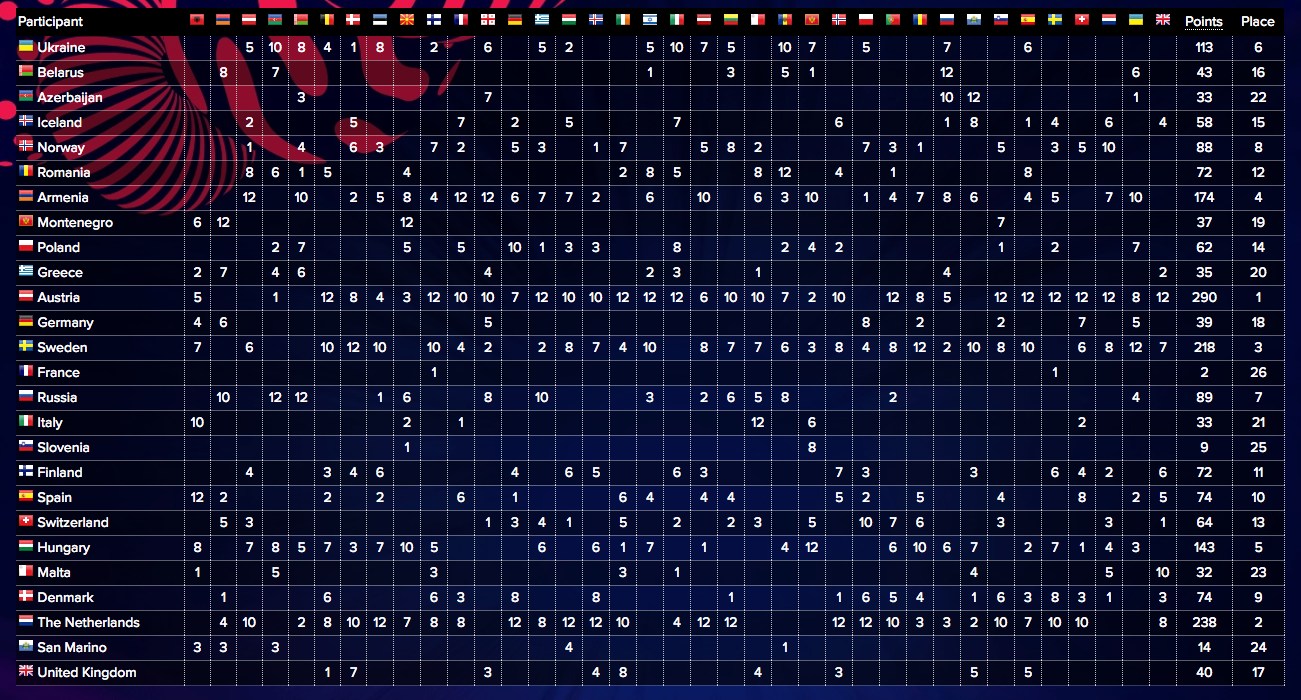
\includegraphics[width=16cm, height=9cm]{./2014Scoreboard}
\caption{2014 Scoreboard}
\label{f_2014Scores}
\end{figure}

This voting system creates a matrix of scores as seen in Figure \ref{f_2014Scores}\cite{EurovisionScoreboard}. The \textit{voters} are arranged along the top alphabetically, while the \textit{participants} are along the left hand side. Points refers to the final total of all the scores received at the end of all voting, and rank is their final position in the competition. 

This is important to look at as it can help clarify what this project's aim is. A solution to the problem is found by swapping the \textit{voters} column along the top into different positions and then analysing the scores after each country has voted, to reach an \textit{entertaining} order for those countries to reveal their votes.

% Your background section should end with a clear statement of the research questions problem your project is trying to answer. 
%These will reflect the aim of your project, but will be different in that they explain the problem you are attempting to solve
Hence the problem that this project is trying to solve is about ordering who votes when so as to maximise some mathematical concept of entertainment.

\clearpage
\section{Algorithm Designs and Approach}\label{AlgorithmDesigns}
% give reader a clear picture of the system
% specification becomes: description of the problem and what is required of a solution
% design becomes: description of your approach to solving the problem and your suggested solution(s)
% problem statement section and then a section describing one or more suggested algorithms to solve the problem
% Later in results and evaluations describe how to design experiments to test how well the algorithms solve the problem and present experimental results with an evaluation of your suggested solutions
% big-O
% reasoning behind writing each algorithm
This section should give an understanding of the main parts that are needed to solve this problem, before implementation can be explained. This will include some pseudocode of the algorithms used, explanations of the neighbourhoods tried and the entertainment functions designed. It is intended to give an introduction to the why and how these parts of the project exists, before Section \ref{Implementation} goes into implementation details with code and explanations using Python.

Firstly to help clarify the problem it is easier to view a much smaller competition and then run through the main points of theory, that are then used in the full Eurovision system.

Firstly we design a competition that involves 4 teams total, of which 2 are \textit{participants}. The scoring system is even more simple than the one used by Eurovision. Here each voting team gives 1 point the team they prefer and 0 to the other. A team cannot give itself 1 point. The scores given in this game are shown in Table \ref{t_simpleMatrix}.

\begin{table}[H]
\centering
\caption{Scores for simple example game}
\label{t_simpleMatrix}
\begin{tabular}{|l|l|l|l|l|}
\hline
        & Germany & France & Spain & Austria \\ \hline
Austria & 1       & 1     & 1      & 0       \\ \hline
France  & 0       & 0     & 0      & 1       \\ \hline
\end{tabular}
\end{table}

From Table \ref{t_simpleMatrix} we can see how the scores will be calculated in this type of competition. For simplicity, the order that the teams vote is the order from left to right in Table \ref{t_simpleMatrix}. This means that after Germany has voted the scores are $Austria: 1, France: 0$, the rest of the competition is shown in Table \ref{t_simpleScores}

\begin{table}[H]
\centering
\caption{Scores per round}
\label{t_simpleScores}
\begin{tabular}{|l|l|l|l|l|}
\hline
        & After Germany's vote & After France's vote & After Spain's vote & After Austria's vote \\ \hline
Austria & 1                    & 2                  & 3                   & 3                    \\ \hline
France  & 0                    & 0                  & 0                   & 1                    \\ \hline
\end{tabular}
\end{table}

We can see that Austria wins this competition, with 3 points. This cumulative scoring extends to the full Eurovision competition in the exact same way, except for in that case there are 30+ voters.

All that is needed to turn this simple example into Eurovision is to add all the \textit{voters} and \textit{participants} and change the scores given out to be $12, 10, 8-1$ instead of just 1 and 0.

\subsection{$\varepsilon$ Functions}\label{EntertainmentFunction}
From this small example it can be seen that the ordering used would not be very entertaining as after the second round of voting, Austria could not lose, only draw. 

To justify this mathematically we could look at the difference between the scores of the two teams at each round (Table \ref{t_simpleDifferences}). By summing that difference over the whole competition we get a difference of \textbf{8}, which represents the order $[Germany, France, Spain, Austria]$. 

\begin{table}[H]
\centering
\caption{Difference per round for first order}
\label{t_simpleDifferences}
\begin{tabular}{|l|l|l|l|l|}
\hline
        & After Germany's vote & After France's vote & After Spain's vote & After Austria's vote \\ \hline
Difference & 1                    & 2                  & 3                   & 2                    \\ \hline
\end{tabular}
\end{table}

However if we swap when Austria and Germany vote we would get a total difference of \textbf{4} over all the rounds (Table \ref{t_simpleDifferences2}). This would intuitively seem like a more entertaining order as well as having a lower total difference.

\begin{table}[H]
\centering
\caption{Difference per round with Germany and Austria swapped}
\label{t_simpleDifferences2}
\begin{tabular}{|l|l|l|l|l|}
\hline
        & After Austria vote & After France's vote & After Spain's vote & After Germany's vote \\ \hline
Difference & 1                    & 0                  & 1                   & 2                    \\ \hline
\end{tabular}
\end{table}

Any entertainment functions ($\varepsilon$ functions) talked about in this section share some characteristics that need to be explained. The first is that they take a \textbf{solution ($\Phi$)} to the problem (see Glossary-3) as input and they return a single \textbf{entertainment value} ($\varepsilon$) (see Glossary-4). Moreover they calculate the \textbf{scores}($S$) (see Glossary-6) for each \textit{participant} country every \textbf{round} ($R$)(see Glossary-5).

\subsubsection{MaxMin}
The first entertainment function that was designed is the one described in the small example at the start of this section, named \textbf{MaxMin}. As it's name suggests it works by finding the difference between the highest score (max) and the lowest score (min) after each voting round. It then sums the value which is the $\varepsilon$ value for that solution. This function follows quite naturally from watching and analysing the Eurovision competition as the way roll-call style voting works, everything is building towards the later end of the voting order. Hence it seems to be a innate part of the competition that you would want every country to be in with a chance of winning as often as possible. Moreover as there is only one prize, for first place, it is even less important to worry about positioning other than the top.

So each round the distance ($\Lambda$) for a set of scores, $S$ is calculated as such:
\begin{equation}\label{lambda}
	\Lambda = \max(S) - \min(S)
\end{equation}

Then keeping the distance per round $i$ as $\Lambda_i$, the entertainment value ($\varepsilon$) is found by:
\begin{equation}\label{epsilon}
	\varepsilon = \sum_{i=0}^{n_R}  \Lambda_i
\end{equation}
(See Glossary-5 for $n_{R}$)

This is a relatively simple equation and hence transfers simply to code. However more importantly, it encodes an intuitive part of entertainment mathematically. This functions encodes the fact that an entertaining competition is one in which the distance between first and last place is as low as possible as often as possible. In this case instead of \textbf{maximising} $\varepsilon$, we want to \textbf{minimise} it.

Over the course of a whole competition i.e: $n_R$ voting rounds, it is intuitive to want that distance to stay as low as possible, by finding the sum of the distance ($\Lambda$) in each round and then using optimisation algorithms to try and find a solution ($\Phi$) that minimises this value.

There is however one major drawback of the basic \textbf{MaxMin} method, which is that in some rounds, especially later in the competition, the last place country is actually mathematically eliminated from the race for first place.

\subsubsection{RefinedMaxMin}
This leads to a second version of the entertainment function for this problem. As it is essentially a refinement of the first function and not a brand new method it is called \textbf{RefinedMaxMin}.

Equation \ref{epsilon} is the same across both functions, however where \textbf{RefinedMaxMin} and \textbf{MaxMin} differ is how the $\min(S)$ part of equation \ref{lambda} is calculated. As some of the countries cannot win the competition after some number of rounds, they should not be taken into account when seeing if a solution is entertaining or not.

To find whether a team can still win, the upper bound of points left available to be given is found. This means that we assume for each team, and for the remaining rounds left to be revealed, that they gain the maximum (12) points and the hence we find the highest score they could ever attain. This method does not take into account whether the country has already given itself a vote (in which case they would not be allowed to get 12 points in that round). This was done to simplify the method and make testing it's improvements against MaxMin easier. Furthermore finding the upper bound is generally safe, especially when removing the low scoring teams in Eurovision as voting is generally quite uniform past a certain point in the voting; i.e countries that are given high points already generally get more, and countries that have received few points continue to get few. Further refinements to this calculation are discussed in Section \ref{FutureWork}.

The method for finding if a team can still win is to first sort the scores for every country in round $i$ in ascending order. Then iterating through that list of scores from the start and for each score checking whether equation \ref{stillWin} is true.
\begin{equation}\label{stillWin}
	countriesScore + (maxScorePerRound * roundsRemaining) <= currentTopScore
\end{equation}

If equation \ref{stillWin} holds true then that country cannot win even if it received the maximum number of points (12 in Eurovision's case) and the leaders received the worst score possible (0), for the remaining voting rounds. As the scores are in ascending order the last minScore found for which Equation \ref{stillWin} held true is the minimum score to be returned.

It is quite simple to justify this refinement when looking at the competition. Those teams who cannot win should not be making a mark on the entertainment of the voting order as most viewers will not be paying attention to their scores and rank. Moreover this refinement only works in competitions where there is only interest at the top of the table as opposed to competitions with relegations or play-offs, where more than just who is the overall winner is important.

It is important to start with the design of the entertainment functions as they are the main workhorse for finding solutions to the problem. The approach to describe them was to analyse the competition and try and identify things in a competition that lead to excitement. From those ideas, it was a case of trying to formalise that theory into a concrete piece of maths that could then be programmed. Furthermore the entertainment functions are quite problem specific and may not transfer well into other problems, whereas the algorithms are entirely agnostic to the problem at hand. This means the entertainment functions follow much more closely from the problem itself than any other part of the project.

\subsection{Neighbourhoods}\label{Neighbours}
An important part of solving optimisation problems is designing and implementing neighbourhoods\cite{Neighbourhood} for given solutions. As a solution ($\Phi$) is a list of \textit{voters} in a certain order, then we define a neighbourhood as any other solution that has two members swapped. This means that there are only two changes between a solution and any of it's neighbours.

In this regard an order is a \textit{permutation} of the \textit{voters}. Using Cauchy's two line notation for permutations\cite{Cauchy}, we can show the basic theory for our neighbourhoods.

\begin{equation}\label{neighbourhood}
\begin{pmatrix}
x_{1} & x_{2} & x_{3} & \cdots & x_{n} \\
\sigma(x_{1}) & \sigma(x_{2}) & \sigma(x_{3}) & \cdots & \sigma(x_{n}) \\
\end{pmatrix}
\end{equation}

Equation \ref{neighbourhood} shows the first solution on the top row and a neighbour of that solution on the bottom row. The functions that map the elements of a solution to a neighbour ($\sigma$) are explained below.

These methods are examples of cyclic permutations i.e a permutation of a set which maps a subset of elements to each other in a cyclic way, while mapping all other elements of the set to themselves. The cyclic parts of a permutation are called \textit{cycles}. A cycle with only two elements is called a \textit{transposition}\cite{cyclicPerm}. As both of the following methods only contains two indexes, they are \textit{transpositions}.

\subsubsection{Random neighbour}
The first idea and most simple for this problem, was to swap two random elements of the ordering. This means that the function $\sigma$ swaps the two elements at those indexes. This method can be described as such in equation \ref{random} for two random indexes $i$ and $j$.

\begin{equation}\label{random}
\begin{split}
	\sigma = x_i \mapsto x_j,\\ x_j \mapsto x_i,\\ \forall x \neq i \lor \forall x \neq j: x \mapsto x
\end{split}
\end{equation}

This means that we swap the elements at indexes $i$ and $j$ and swap the rest with themselves. The code for this will be explored in Section \ref{Imp-Neighbours}. This method gives a large set of possible neighbours as theoretically for any single solution there are \{length of solution $\times$ length of solution - 1\} possible neighbours. In the 2014 Eurovision competition this would mean $\{37 \times 36 = 1332\}$ neighbours.

This method may be simple, however, when a closer look is taken at the actual $\varepsilon$ values of solutions that are very similar to each other i.e they have 3 or 4 elements swapped and most elements the same, it is clear that their $\varepsilon$ values only differ by a little. This calls into question if the method detailed above is actually going to help the optimisation algorithm reach an optimal solution.

\subsubsection{Adjacent neighbour}
The questions about the efficacy of the random method leads to another method for finding a neighbour of a solution. As solutions that are close together are usually quite similar, it is intuitive that swapping adjacent elements may improve the solutions found.

This method works by finding a random value between 0 and length of solution - 1. Then swapping the element at that index with its immediate neighbour to the right i.e. index + 1. It can be expressed in the same way as in equation \ref{random}, except that in this case index $i$ is a random number and index $j = i + 1$.

Another difference between this method and the random method is how it can actually be calculated. After finding a neighbour of a given solution, the $\varepsilon$ value of that solution must be found. By swapping 2 adjacent countries in the solution a \textit{partial re-calculation} of the entertainment value can be done using the entertainment value of the previous solution. 

As the previous solution and the new solution only differ by one position it is possible to only partially re-calculate the $\varepsilon$ value. This idea is implemented separately to the \textbf{MaxMin} and \textbf{refinedMaxMin} methods in the code, and explanation as to how can be found in Section \ref{Imp-Ewrappers}.

Re-calculation involves removing the distances of the swapped countries in the old solution and adding them back in their new positions in the new solution. The equation for this is shown in \ref{Recalc}.

\begin{equation}\label{Recalc}
	\varepsilon_{new} = \varepsilon_{old} - \Lambda_{ij_{old}} + \Lambda_{ij_{new}}
\end{equation}

The $\varepsilon_{new}$ and $\Lambda_{ij_{old}}$ values can be found by keeping them from the old solution and passing them into the next $\varepsilon$ calculation function. The $\Lambda_{ij_{new}}$ must still be re-calculated however only up to the higher of the two indexes.

The efficacy of this neighbourhood can be see when calculating the $\varepsilon$ values. A full calculation, such as is used in the random swap method involves \{number of voters $\times$ number of participants\} or $V \times P$. 

However due to the adjacency of the swaps Table \ref{scoreCalcsAdj} shows what this method needs to calculate.

\begin{table}[H]
\centering
\caption{Score calculations needed with adjacent neighbour}
\label{scoreCalcsAdj}
\begin{tabular}{|l|l|}
\hline
        & Number of calculations \\ \hline
Max     & $V \times P$           \\ \hline
Min     & $2 \times P$           \\ \hline
Average & $\approx 18 \times P$          \\ \hline
\end{tabular}
\end{table}

Table \ref{scoreCalcsAdj2014} show that what this would mean in the 2014 competition.
\begin{table}[H]
\centering
\caption{Approximate 2014 Eurovision specific calculations}
\label{scoreCalcsAdj2014}
\begin{tabular}{|l|l|}
\hline
        & Number of calculations \\ \hline
Max     & 962                    \\ \hline
Min     & 52                     \\ \hline
Average & 468                    \\ \hline
\end{tabular}
\end{table}

A deeper comparison and evaluation between the two methods can be found in Section \ref{OtherTesting}

\subsection{Optimisation Algorithms}\label{Algorithms}
In the previous section the necessary first steps to solve the problem were outlined. Namely calculate an entertainment value ($\varepsilon$) which can be optimised. To do this optimisation it is necessary to use a set of optimisation algorithms which maximise or minimise a value in order to settle on an optimal solution.

\subsubsection{Greedy Search}
The first algorithm that was posited was a simple Greedy search algorithm. Greedy search works on the idea that by selecting the optimal choice at every possible stage, it will lead to a globally optimal solution.\cite{GreedySearch}

At first glance it is not obvious to see if the problem we are attempting is simple or complex. This lead to Greedy search as a good first try as it is sufficiently simple so that the code is easy to write and more importantly it will likely find the optimal solution if the solution space is simple. If the solution space \textit{is} in fact too complex then Greedy may still find a good approximate solution.

An important point to re-iterate, as mentioned when talking about the $\varepsilon$ functions, is that even though in the report it may be mentioned that the algorithms are \textbf{maximising} entertainment to do this in the code, we have to \textbf{minimise} the $\varepsilon$ value produced by the $\varepsilon$ functions. All algorithms described in this report follow this methodology.

The pseudocode for Greedy is shown in Algorithm \ref{greedyPseuodocode} in the appendix.

As can be seen, it is a very simple algorithm that takes possible solutions and compares them to the already found best solution. It's simplicity is, unfortunately, also it's downfall in this problem. Although it can find a good approximate solution it is not able to find optimal solutions that other algorithms do find.

The stopping criterion is part of both Simulated Annealing's and Greedy search's algorithm. The stopping criterion defines when the algorithms should stop. To maintain parity between the algorithms, the stopping criterion chosen was to stop when a certain number of iterations had passed without a new solution being found. The value of the stopping criterion is given by the variable $num\_iterations$ in both algorithms implementations and pseudocode, and to achieve this idea it is necessary to reset the value of $i$ when a new solution is found. This can be seen on line 10 of Algorithm \ref{greedyPseuodocode}

Looking at the pseudocode, and with some simplifying assumptions the worst case time complexity for this Greedy search algorithm can be found.

This is done by giving all the instructions that make a difference to complexity, a value $T_i$ from their line number. This means line 5 is $T_5$, then working out how many times that instruction will need to be run given an input. The input is the \textit{voters} and \textit{participants}, $V$ and $P$. Some lines can be ignored as they do very little to complexity. Table \ref{greedyLines} shows the complexity added by some important lines.

\begin{table}[H]
\centering
\caption{Worst case Greedy complexity per line}
\label{greedyLines}
\begin{tabular}{@{}|l|l|@{}}
\toprule
Line               & Effect on complexity                                                                        \\ \midrule
$T_1$              & run once with $V$ steps                                                                     \\ \midrule
$T_2$              & run once                                                                                    \\ \midrule
$T_3$              & run once with $V \times P$ steps                                                            \\ \midrule
$T\_5$             & $m$ times with constant steps                                                               \\ \midrule
$T\_6$             & $m$ times with $V \times P$ steps; as worst case, assume that full re-calculation is needed \\ \midrule
$T\_7 - T\_{11}$ & $m$ times as is worst case, so assume this block always run                                 \\ \midrule
$T_{12}$           & $m$                                                                                         \\ \midrule
$T_{14}$           & $1$                                                                                         \\ \bottomrule
\end{tabular}
\end{table}

\textbf{N.B} The main loop (lines 4 - 13) is constant, given it comes from \textit{num\_iterations}. It adds $m$ times to the instructions inside it.

Factoring this down into equation \ref{greedyComp} gives: 

\begin{equation}\label{greedyComp}
\begin{aligned}
	f(n) ={} & \ (V \times T_1) + T_2 + (V \cdot P \times T_3) + (m \times T_5) + (m \times V \cdot P \times T_6) \\
	 	& + (m \times T_{7 - 11}) + (m \times T_{12}) + T_{14}
\end{aligned}
\end{equation}

From this we can safely ignore anything that is less than the highest order as it will dominate the complexity growth. Moreover we can see that the highest order is $T_6$, so we are left with equation \ref{greedyCompSimp}

\begin{equation}\label{greedyCompSimp}
\begin{aligned}
	f(n) ={} & \ (m \times V \cdot P \times T_6) \approx m \times V \cdot P
\end{aligned}
\end{equation}

where $P <= V \ll m$. This can be further simplified in terms of \textit{voters} ($V$), as $P$ is always less than or equal to $V$ and $m$ is always larger or equal to $V$, they can be roughly equated to $V$. The coefficients of $m$ and $P$ compared to $V$ do not matter to the complexity, just that they are near the same size. This leaves us with a fair approximation of the complexity in equation \ref{greedyCompFinal}.

\begin{equation}\label{greedyCompFinal}
\begin{aligned}
	O(n) \approx{} & \ m \times V \cdot P \approx V \times V \times V \approx O(V^3)
\end{aligned}
\end{equation}

A discussion and comparison with the other algorithms can be found in Section \ref{OtherTesting}.\footnote{A full table of Big-O complexity for all algorithms can be found in the appendix in table \ref{bigO}}

\subsubsection{Brute force}
After running the Greedy algorithm and collecting some initial results it became clear that it would be difficult to know by just looking at the problem, what a good $\varepsilon$ value would be. This lead to the discussion about using a Brute force algorithm to try and enumerate all the solutions.

The idea is extremely simple, try all possible solutions and keep track of the best found. Even though the pseudocode and the real code will differ, the pseudocode help understand the algorithm so is shown in Algorithm \ref{bruteForcePseudocode}

When some simple calculations are made about the solution space it is clear as to why the Brute force method is not ever going to feasible for this problem. Searching all solutions, is not a simple task. As it must look at all permutations of solutions which are of length $V$, the complexity of Brute force follows the number of permutations for n distinct objects.\cite{Permutation}. This is shown in equation \ref{bruteComp}.

\begin{equation}\label{bruteComp}
\begin{aligned}
	O(n) \approx{} & \ O(V!)
\end{aligned}
\end{equation}

This means that in all cases Brute force will run in $\approx V!$ time. Comparison to the other algorithms used can be found in Section \ref{OtherTesting}.\footnote{A full table of Big-O complexity for all algorithms can be found in the appendix in table \ref{bigO}}

For example in the 2014 running of Eurovision this would be $37!$ which, after approximating the time to look at one single solution, would take about $1.2\times10^{40}$ seconds, which is quite obviously computationally infeasible with the time and resources for this project.

\subsubsection{Simulated Annealing}
The performance of Greedy and Brute force reveal the fact that this problem is not a simple one at all and hence another, more capable algorithm is needed to find more optimal solutions. To do this the Simulated Annealing algorithm\cite{Kirkpatrick} was used.

The pseudocode for Simulated Annealing can be found in Algorithm \ref{simAnnealingPseudocode} in the appendix. It is quite a lot more complex than either Brute force or Greedy search.

The skeleton of the algorithm is shared with both the previous algorithms; that is, lines 22 - 25 in Algorithm \ref{simAnnealingCode} are the same as lines 5 - 7 in Algorithm \ref{bruteForcePseudocode} (Brute force) and lines 9 - 12 in Algorithm \ref{greedyPseuodocode} (Greedy).

The important part where they differ is how they pick a solution to try. Simulated Annealing finds a neighbour of the current solution, however where Greedy always takes that solution and compares it to the best, Simulated Annealing does two things before that comparison.

Firstly as can be seen on lines 12 - 14 of Algorithm \ref{simAnnealingPseudocode}, it checks whether the new solution is better than the current one. If it is better, then it takes that solution for comparison to the best. However, if it is not better there is still a chance Simulated Annealing will take it for comparison. 

In lines 16 - 19, a check is performed that allows worse solutions than the current to be checked against the best. This is usually called an \textit{"Uphill move"} as, if $\varepsilon$ values of solutions are plotted then better solutions are nearer to 0 and worse moves are further, meaning they will be moving upwards on the curve as can be seen in Figure \ref{uphillMove}.

\begin{figure}[H]
\centering
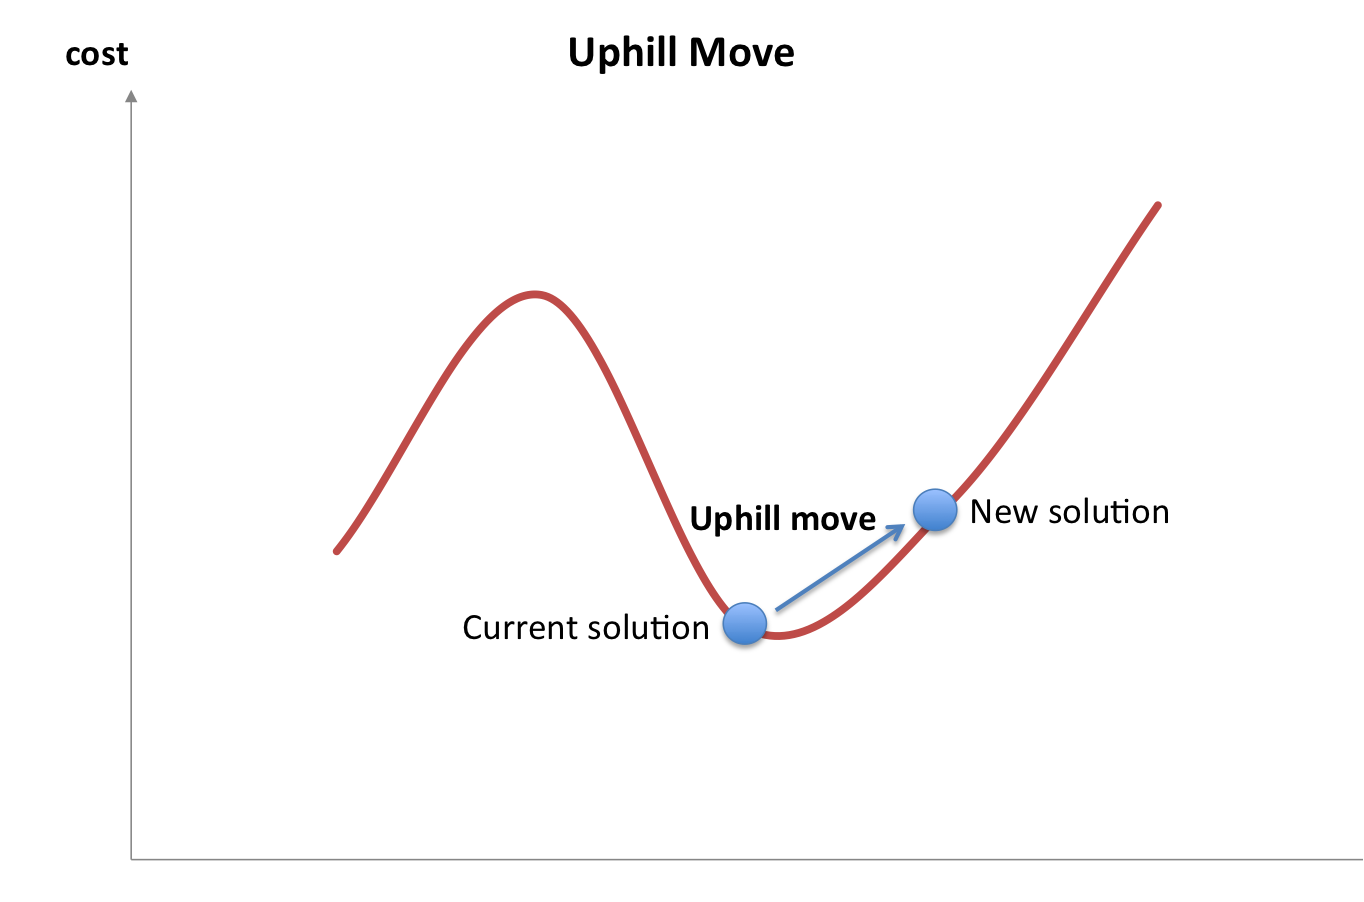
\includegraphics[width=16cm, height=9cm]{./uphillmove}
\caption{Uphill moves in optimisation problems}
\label{uphillMove}
\end{figure}

The reason for accepting a worse solution is because it allows for a more extensive search for the optimal solution. Line 17 is a feature that is designed to prevent the algorithm from becoming stuck at a local minima that is worse than the global one\cite{simAnnealing}. The local minima is represented by the bottom of the red curve in Figure \ref{uphillMove}. Moreover as the likelihood of accepting a worse solution varies with the value of $t$, it allows the algorithm to take worse solutions at the start, but not take the worse solution nearer the end, meaning the \textit{"Uphill moves"} occur so that the algorithm does not get stuck in a local optima early.

Another part that is specific to Simulated Annealing is the concept of the cooling schedule. The values that make it up are $ti$, $tl$ and $cr\_coefficient$. $ti$ is the initial temperature and should be high enough so that the final solution is independent of the initial solution, and so that it encourages a wide exploration of the feasible solutions at the start. $tl$ is the number of iterations that occur at each temperature and the $cr\_coefficient$ is the rate at which the temperature is reduced.\cite{coolingSchedule}

An approximation of the worst case Big-O of Simulated Annealing is shown in Table \ref{simLines}.

\begin{table}[H]
\centering
\caption{Simulated Annealing complexity per line}
\label{simLines}
\begin{tabular}{@{}|l|l|@{}}
\toprule
Line              & Effect on complexity                                                                                                        \\ \midrule
$T_1$             & run once with $V$ steps                                                                                                     \\ \midrule
$T_2$             & run once with $V \times P$ steps                                                                                            \\ \midrule
$T_3$             & run once with constant steps                                                                                                \\ \midrule
$T_4$             & run once with $V \times P$ steps                                                                                            \\ \midrule
$T_7$             & $m \times l$ times with constant steps                                                                                      \\ \midrule
$T_8$             & $m \times l$ times with $V \times P$ steps                                                                                  \\ \midrule
$T_9$             & $m \times l$ times with constant steps                                                                                      \\ \midrule
$T_{10} - T_{19}$* & $m \times l$ times with constant steps \\ \midrule
$T_{20} - T_{23}$ & $m \times l$ as it is the worst case, the assumption is that this block is always run                                       \\ \midrule
$T_{26}$          & $m$ times with constant steps                                                                                               \\ \midrule
$T_{27}$          & $m$ times with constant steps                                                                                               \\ \midrule
$T_{29}$          & run once                                                                                                                    \\ \bottomrule
\end{tabular}
\end{table}

* This if-else block can be treated as one because one of the two blocks will always be run

\textbf{N.B} The main loop (lines 5 - 28) is constant, given it comes from \textit{num\_iterations}. It adds $m$ loops to the instructions inside it. The inside loop (lines 6 - 25) is also constant, given it comes from the temperature length, \textit{tl}. It adds $l$ times to the instructions inside it.

Factoring this down into equation \ref{simAnnComp} gives: 

\begin{equation}\label{simAnnComp}
\begin{aligned}
	f(n) ={} & \ (V \times T_1) + (V \cdot P \times T_2) + T_3  + (m \times V \cdot P \times T_4) \\
	 	& + (m \times l \times T_7) + (m \times l \times V \cdot P  \times T_8) + (m \times l \times T_9) \\
		& + (m \times l \times t_{10 - 19}) \\
		& + (m \times l \times T_{20 - 23}) \\
		& + (m \times T_{26}) + (m \times T_{27}) + T_{29}
\end{aligned}
\end{equation}

From this we can safely ignore anything that is less than the highest order as it will dominate the complexity growth. Moreover we can see that the highest order is $T_8$, so we are left with equation \ref{simAnnCompSimp}

\begin{equation}\label{simAnnCompSimp}
\begin{aligned}
	f(n) ={} & \ (m \times l \times V \cdot P \times T_8) \approx m \times l \times V \cdot P
\end{aligned}
\end{equation}

where $P <= V <= l <= m$. As before this can be further simplified in terms of \textit{voters} ($V$). In this case, there is an extra term with will be greater than or equal to $V$. This leaves us with a fair approximation of the complexity in equation \ref{simCompFinal}.\footnote{A full table of Big-O complexity for all algorithms can be found in the appendix in table \ref{bigO}}

\begin{equation}\label{simCompFinal}
\begin{aligned}
	O(n) \approx{} & \ m \times l \times V \cdot P \approx V \times V \times V \times V \approx O(V^4)
\end{aligned}
\end{equation}

A full comparison between the algorithms and their complexities is undertaken in Section \ref{OtherTesting}.


\subsubsection{Piecemeal}
Part way through the project a slightly different approach to building a solution was suggested. The three algorithms discussed above all have a major thing in common, that they move from a \textbf{full} solution to another. It was suggested that another methodology for finding a solution could be used. The development of this algorithm was not directly due to the performance of the other algorithms. At this time in the project Simulated Annealing was performing very well; the decision to design this algorithm was more influenced by gaining a deeper understanding of the problem and the entertainment functions that had been designed. The Piecemeal method shares some of its theory with Constraint Satisfaction Problems (CSP's)\cite{CSP} and more specifically backtracking algorithms used within them\cite{backtracking}. Backtracking algorithms contain the idea to incrementally build a full solution by trying different partial solutions.

This method begins with just one \textit{voter} instead of a full solution. This \textit{voter} can be found randomly or just be the first in the list. Then to pick the next \textit{voter} to add to the solution, the algorithm looks at all the available \textit{voters} it could add and it picks the one that gives the lowest overall $\Lambda$ value. The $\Lambda$ value is the distance between the best and worst who can still win. At the end this value is summed to get the solution's $\varepsilon$ value.

It adds the best next \textit{voter} to it's current solution until it reaches a full solution. Whereas the search methods, such as Greedy and Simulated Annealing, keep track of a set of possible \textbf{full} solutions, this method named the \textit{Piecemeal} method, builds a solution by doing a greedy search of the available next \textit{voters} that could be added.

This method hopes that by picking the best possible next choice this will lead to a good approximation or globally optimal solution. It acts very much like Greedy search that has been discussed, and the pseudocode supports that, however by working on partial solutions instead of full solutions, the idea is that it will at least approximate a good solution without having the need to check many full solutions, hence increasing performance, especially for large solution problems.

The pseudocode for it is shown in Algorithm \ref{piecemealPseudocode} and the implementation is discussed in more detail in Section \ref{Imp-Piecemeal}.

The main points of interest are that even though lines 7 - 9 look very similar to the three algorithms discussed before, there is a subtle difference. In this algorithm, the value that is being checked against the best is not entertainment ($\varepsilon$) but the distance ($\Lambda$).

Another point of interest is a more academic one. It is a question of choosing which \textit{voter} to put at the start. The two most obvious choices are randomly choosing one, which complicates the code slightly, or picking the first from the given list of voters, making the code simpler. The choices of first \textit{voter} and their effect on the $\varepsilon$ returned is explored more in Section \ref{solutions}.

To come to a solution, the algorithm must look at a descending number of possible next solutions from the length of the solution down to 1. In the 2014 Eurovision, this would be 37 choices in the first round, 36 in the second, 35 in the third etc. until all \textit{voters} are accounted for.

The formula in equation \ref{infiniteSeries} describes the worst case that this algorithm will take. This can be represented as a triangular number\cite{triangularNumber} as it is the sum of the natural numbers from 1 to $V$.

\begin{equation}\label{infiniteSeries}
	O(n) = \sum_{k=1}^{V} k =  V + (V-1) + (V-2) + ... + 1 \approx \frac{V(V+1)}{2}
\end{equation}
which can then be simplified for Big-O notation into equation \ref{bigOPiecemeal}. This is because for looking at the complexity of algorithms it is most interesting to look at the term that does the most to the complexity, so in this algorithms case it is the $V^2$ term.\footnote{A full table of Big-O complexity for all algorithms can be found in the appendix in table \ref{bigO}}

\begin{equation}\label{bigOPiecemeal}
	O(n) = \frac{V(V+1)}{2} = \frac{V^2 + V}{2} \approx V^2 + V \approx O(V^2)
\end{equation}

Looking at the Big-O complexity in equation \ref{bigOPiecemeal} and comparing it to the others is done it Section \ref{OtherTesting}.

% piecemeal example failing

\section{Implementation of System}\label{Implementation}
% describes system but does so at finer level of detail, down to code level
% realisation of concepts and ideas developed earlier
% complete source code should be provided separately
% pick out and describe pieces of code which for example:
% are especially critical in operation of system
% are of particular interest
% illustrate a non-standard or innovative way of implementing an algorithm, data structure
% mention unforeseen problems that you encountered when implementing the system like:
% difficulties involving existing software
% lack of suitable supporting framework
% over ambitious project aims
% A seemingly disproportionate amount of project time can be taken up in dealing with such problems. The Implementation section gives you the opportunity to show where that time has gone.
In this section, the main parts of the project's code will be explored. This will take the theory and pseudocode described in Section \ref{AlgorithmDesigns} and discuss the actual code implemented as part of the project. It will both discuss some specific code as well as a discussion as to why parts of the system were implemented in certain ways. All code referenced in this section can be found in the attached source code files, submitted along with this report.

\subsection{$\varepsilon$ function wrappers}\label{Imp-Ewrappers}
The $\varepsilon$ functions form one of the most important parts of this project, however for them to be implemented they need some contextual data. The functions described below are larger functions that wrap around and allow the $\varepsilon$ functions to do their work. The $\varepsilon$ functions actually form just the $min(S)$ part of equation \ref{lambda}. 

These wrapper functions share an important part, which is shown in \ref{findScores}.\footnote{Section of code from \textbf{getEntertainment} in \textit{support.py}. Full function can be found in attached source code}

\begin{figure}[H]
\caption{Calculating the cumulative scores per participant}
\label{findScores}
\begin{lstlisting}
for j in range(len(solution)):
  for i in range(len(countries)):
    v = voters.index(solution[j])
    scores[i] = scores[i] + score_board[i][v]
    ...
\end{lstlisting}
\end{figure}

The main point of interest is the two nested \textit{for} loops and specifically lines 3 and 4.

As the distance ($\Lambda$) is found as the difference between max and min scores in each round, it is necessary to go through and cumulatively add the scores given to each \textit{participant} in every round. This is stored in the array $scores$ at the index for that \textit{participant}: $scores[i]$. The $score\_board$ is the matrix of all scores given, as discussed in Section \ref{Background}. 

These lines are interesting to highlight as they are likely the most critical lines in all the system. Every algorithm must use them at some point and all $\varepsilon$ functions will need them to calculate the $\varepsilon$ value.

As the score lookup is done against a matrix of scores, it is necessary to find the correct column to look in. The row is the current \textit{participant}: $i$, however finding the column is a little more complex. 

The columns in the matrix are in a certain order, alphabetical in the case of the 2014 Eurovision dataset. This, along with the fact that each solution is a permutation of that order, means that the currently voting country in the solution, $solution[j]$, must be found in the original order to correctly retrieve the score it gives. By keeping track of the original order as it corresponds to the scoreboard, the system only ever has to keep one matrix in memory, along with 2 list (of \textit{voters} and \textit{participants}). Any other method would include shuffling the scoreboard into the order of the current solution. As the scoreboard grows i.e in other, larger problems, this method would become untenable and possibly begin adversely affecting the algorithm's runtimes and complexities.

The method $array.index(element)$ returns the index in the given $array$ of the given $element$. In this case $solution[j]$, would be a country name such as "Germany", and the value of $v$ will be an integer corresponding to the column.

Looking at the full code listings there are actually two methods that wrap around $\varepsilon$ calculation functions to provide them with context and data. These are called \textbf{offsetGetEntertainment} and \textbf{getEntertainment}, and they both share the code shown in Figure \ref{findScores}. They are also fully independent of the \textit{maxMin} and \textit{refinedMaxMin} functions which are the actual $\varepsilon$ functions. These methods differ because of when and why they can be used.

The main reason for these differences is shown in Section \ref{Neighbours}, as using different neighbourhood methods leads to different ways to calculate the entertainment. 

\subsubsection{offsetGetEntertainment}
Firstly the more complex \textbf{offsetGetEntertainment}\footnote{Can be found in \textit{support.py} in source code} is used in conjunction with adjacent neighbour swaps as it relies on using the previous $\varepsilon$ value. The theory behind why this works is explained in Section \ref{Neighbours}, specifically the Adjacent neighbours subsection and equations \ref{random} and \ref{Recalc}.

This function is shown in Figure \ref{offsetGetEntertainment} in the appendix.

The important parts to understand about this implementation are, that for it to work it must be given three things. Two keys that correspond to the indexes of the \textit{voters} that were swapped to get this solution; the $\varepsilon$ value of the old solution, and the array of the distances used to calculate that solution's $\varepsilon$ value.

One obvious point of difference is between the \textit{for} loops in Figure \ref{offsetGetEntertainment} and Figure \ref{findScores}. In the \textbf{offsetGetEntertainment} method the \textit{for} loops only need to calculate the scores up to the higher of the two keys as the scores after the swaps are unchanged.

There are some further parts that need explanation. The actual recalculation described in Equation \ref{Recalc} is implemented in line 20. On lines 3 and 4, a copy of $countries$ and $solution$ are taken using Pythons array copy syntax. This is most likely not really necessary but during implementation there was a couple of times where after amending one of the lists locally inside a method, the global version of that list that should have stayed the same, was also changed. This is a little hack that means that any local version of the lists that are amended will not override the original. This small problem is further discussed in \ref{Eval}.

Lines 22 and 23 are necessary so that the new distance values can be passed to this function again, with the distances in the correct positions. Essentially what this does is constantly pass around a list of distances, amending it by swapping values before passing it on.

\textbf{offsetGetEntertainment} is certainly faster and more performant for most solutions. This does depend on where in the solution the swaps have taken place (explored in Section \ref{OtherTesting}.) The main drawback of this method is that is can only be used with adjacent neighbourhood and not the random neighbourhood method.

\subsubsection{getEntertainment}
The second entertainment function wrapper is simpler than {offsetGetEntertainment}. \textbf{getEntertainment}\footnote{Can be found in \textit{support.py} in source code} is the general purpose wrapper for calculating the entertainment of a given solution. It can work with either of the two neighbourhoods described. This makes it more general purpose, however it also make it slower especially when the solution size is large.

The points of interest here are found in lines 13, 14 and 15 of Figure \ref{getEntertainment}. These lines implement that which can be found in Equations \ref{lambda} and \ref{epsilon} exactly as described. Line 13 finds the difference between the max of the scores and whatever min was returned by the current $\varepsilon$ function. Line 14 adds the $\Lambda$ value found to an array and then line 15 sums all the $\Lambda$ values found to finally get a $\varepsilon$ value. To allow it to interact with the \textbf{offsetGetEntertainment} method it also keeps track of the array of $\Lambda$ values and returns them so they can be passed to \textbf{offsetGetEntertainment} in the next iteration.

Some test that compare and contrast these two methods can be found in Section \ref{OtherTesting}.

\subsection{$\varepsilon$ functions}\label{Imp-eFunctions}
The \textbf{refinedMaxMin}\footnote{Can be found in \textit{support.py} in source code} method is the more interesting of the two $\varepsilon$ functions to look at in depth. The original \textbf{maxMin}\footnote{Can be found in \textit{support.py} in source code} method is very simple and uses the Python in-built \textit{min()} \cite{PythonMin} method. Both methods use the \textit{max()} \cite{PythonMax} method from Python.

As can be seen in Figure \ref{getEntertainment} on line 12, the \textbf{refinedMaxMin} method is invoked, with the current list of scores for all \textit{participants}, the current solution being tested and what round of voting the competition is at, $j$. The $maxScorePerRound$ is used so that different competitions can define what it is instead of keeping it locally in the function allowing this method to be easily re-used.

The function is shown in Figure \ref{refMaxMin}

\begin{figure}[H]
\caption{refinedMaxMin method}
\label{refMaxMin}
\begin{lstlisting}
def refinedMaxMin(scores, solution, j, maxScorePerRound):
  sorted_scores = sorted(scores[:])
  currentTop = sorted_scores[-1]
  minScore = sorted_scores[0]
  del sorted_scores[-1] # remove highest score
  roundsRemaining = (len(solution) - 1 - j)

  for score in sorted_scores:
    if score + (maxScorePerRound * roundsRemaining) <= currentTop:
      minScore = score
  return minScore
\end{lstlisting}
\end{figure}

The theory behind this method was described in Section \ref{EntertainmentFunction}. Some of the implementation points to pick up on are, line 1 where the in-built Python function $sorted()$\cite{PythonSorted} is used to take the list of scores and sort them in ascending order. This does slow the method slightly, taking the method's complexity to $n \log n$ but it also simplifies the logic later on as the method does not need to keep track of anything other than the minimum found and also only needs to update it.

This implementation is likely not the most efficient way of finding the refined version of the minimum, however it is quite a simple method. 

An important part of the two methods is their Big-O complexity. The complexities are shown in Table \ref{maxMinComp}. The main point to recognise is that the methods are different in terms of complexity which can help in evaluation such as in Section \ref{Results}. The refined method is actually very similar to \textbf{maxMin} except for the sorting step which increases the complexity.

\begin{table}[H]
\centering
\caption{Big-O of $\varepsilon$ methods}
\label{maxMinComp}
\begin{tabular}{|l|l|}
\hline
              & Big-O time complexity \\ \hline
maxMin*  & O(n) \\ \hline
refinedMaxMin & O(n log n)               \\ \hline
\end{tabular}
\end{table}
* Complexity of Python's $min()$ function from\cite{PythonComplexities}

More in depth comparisons between the two methods can be found in Section \ref{OtherTesting}, which take into account the complexity and the minimum scores that the methods produce.

\subsection{Neighbourhood Functions}\label{Imp-Neighbours}
The random and adjacent neighbourhood methods, \textbf{getNeighbour} and \textbf{getAdjacentNeighbour} are very similar to each other as can be understood from the theory in Section \ref{Neighbours}. Both can be found in \textit{support.py}  in the attached source code. This does mean they could be written as one single method which are supplied the keys needed to perform the swaps. This approach \textit{was} given some thought during their implementation however in the end it was decided to favour duplication over complexity in the system. This means that there \textit{are} two methods that are for all intents and purposes exactly the same, but are named differently.

The methods are shown in Figures \ref{adjacentNeighbour} and \ref{randomNeighbour}.

The only difference occurs on lines 3 and 4 in the methods. Firstly in the adjacent neighbour method the first key is found by getting a random integer between 0 and 2 elements from the end of the list. It must be 2 elements from the end as the second key is taken as the first key + 1. In terms of a list this means the element directly to key1's right. The $len(neighbour)$ part is using Python's in-built length function to calculate the length of the list and hence the last index it can return for correct swapping.\cite{PythonLen}.

The random neighbour method uses the Python \textit{random} library in line 3 of Figure \ref{randomNeighbour} to sample the given order and get two random elements back.\cite{PythonSample}. As this method actually returns the elements and not indexes of those elements, like in the adjacent method, it is necessary to change them back into indexes (line 4) for efficient swapping in line 5.

\begin{figure}[H]
\caption{getAdjacentNeighbour method}
\label{adjacentNeighbour}
\begin{lstlisting}
def getAdjacentNeighbour(xNow):
  neighbour = xNow[:]
  key1 = random.randint(0, len(neighbour) - 2)
  key2 = key1 + 1
  neighbour[key2], neighbour[key1] = neighbour[key1], neighbour[key2]
    
  return neighbour, key1
\end{lstlisting}
\end{figure}

\begin{figure}[H]
\caption{getRandomNeighbour method}
\label{randomNeighbour}
\begin{lstlisting}
def getNeighbour(xNow):
  neighbour = xNow[:]
  key1, key2 = random.sample(list(neighbour), 2)
  index1, index2 = neighbour.index(key1), neighbour.index(key2)
  neighbour[index2], neighbour[index1] = neighbour[index1], neighbour[index2]
    
  return neighbour
\end{lstlisting}
\end{figure}

\subsection{Simulated Annealing and Greedy Search}\label{Imp-searchAlgos}
The implementation of the search algorithms is not the most interesting part of this project and hence only a little time will be spent explaining their implementation. Both Simulated Annealing and Greedy Search can be found in the appendices, and in the attached source code in the files \textit{simulatedAnnealing.py} and \textit{greedySearch.py}.

The main reason for not going into depth about their implementations is that both algorithms are essentially general search algorithms that receive the problem specific input from the other functions already described such as \textbf{getEntertainment} and \textbf{getAdjacentNeighbour}.

A point that is shared across both implementations is the increasing while loop that gets reset to 0 when a new solution has been found. Using Greedy Search as an example, in Figure \ref{greedyCode}, the while loop starts at line 10 with $i$ equal to 0. It is incremented on line 22 after an iteration and comparison of a new solution. On line 18, the value of $i$ is reset to 0. This allows the $num\_iterations$ loop to be the number of iterations since a new best solution was found instead of a hard number of loops to go through. This minor implementation detail actually has a very measurable impact on the speed of the algorithms. Due to the nature of the problem space, it is likely that both Greedy search and Simulated Annealing reach local (possibly global) optima. When this happens, they are not going to choose a new solution. Furthermore having the $num\_iterations$ variable set as a hard number of iterations would require a very deep knowledge of the problem space and how the algorithms are traversing it; so that there is little overhead after they have found the best solution they are going to find. This is not really possible so this method also allows for slightly more flexibility.

Another implementation point that is shared is the fact that both algorithms must pass the $oldEntertainment$ and $oldDistances$ into the \textbf{offsetGetEntertainment} method. The reason for this is explained in Section \ref{Imp-Ewrappers}. This also explains the need for the variable $key1$ to be returned from the \textbf{getAdjacentNeighbour} method. 

A minor point that is related to Python as a language is the ability to return multiple values from a function in a tuple by default. This hugely simplifies the code as methods can then return both a neighbour and the first key used to find it (\textbf{getAdjacentNeighbour}) or a possible solution and the individual distances that make up that solution (\textbf{offsetGetEntertainment}). In other languages there are ways to work around this problem, but this solution is one simple way in Python.

Specifically looking at the Simulated Annealing code in Figure \ref{simAnnealingCode}, the main lines of interest in terms of implementation are line 32 and 34. Line 32 uses the Python \textit{random}\cite{PythonRandom} library to get a random number between 0 and 1. It then uses the Python \textit{math}\cite{PythonMath} library to do the $e^{-deltaC/t}$ part that is necessary for Simulated Annealing to work. These again, are two examples of the Python libraries making implementation very simple for this project.

The general cooling ratio values which were explained in Section \ref{Algorithms} on Simulated Annealing, were experimented with throughout the project. The final values are shown in Table \ref{coolingValues} in the appendix and the implementation details are quite self explanatory.

\subsection{Brute force}\label{Imp-Brute}
The implementation for the Brute force\footnote{Can be found in \textit{bruteForce.py} in the attached source code} algorithm was one of the most simple, and this has much to do with the libraries that Python provides. The library used for the Brute force implementation is \textit{itertools}\cite{PythonItertools}, which provides a set of common methods such as \textit{permutations}\cite{PythonPermutations}. This makes this implementation extremely simple as I did not have to write any code to correctly permute through the possible solutions without repetitions, as the library handled it for me. It can be seen on line 5 of Figure \ref{bruteForce}.

\begin{figure}[H]
\caption{Brute Force algorithm implementation in Python}
\label{bruteForce}
\begin{lstlisting}
def bruteForce(score_board, countries, voters):
  best = voters[:]
  bestCost = support.getEntertainment(voters, countries, score_board, voters)

  for solution in itertools.permutations(voters):
    currentCost, dist = support.getEntertainment(solution, countries, score_board, voters)

    if currentCost < bestCost:
      best = solution[:]
      bestCost = currentCost

  return best, bestCost
\end{lstlisting}
\end{figure}

The implementation shares many similarities with the other algorithms described so far. Namely, the if block on line 8 - 10 that checks if the current solution is better than the best found so far. Furthermore it uses the same \textbf{getEntertainment} method that is used by both the other search algorithms described so far. One small but important point is that, in contrast to Greedy and Simulated Annealing, during the main for loop (lines 5 - 10) in Figure \ref{bruteForce}, Brute force cannot use the \textbf{offsetGetEntertainment} method. This is the one drawback of using the \textit{itertools} library. As it controls getting a new solution to try, the key needed for \textbf{offsetGetEntertainment} to work cannot be passed around. This further slows this Brute force implementation.

\subsection{Piecemeal algorithm}\label{Imp-Piecemeal}
The Piecemeal algorithm is the only break from the traditional style of search algorithms that have so far been discussed. Moreover it is the most novel approach to solving this problem in this project.

The theoretical differences were discussed in detail in Section \ref{Algorithms}. The code for this algorithm is shown in Figure \ref{piecemealCode} in the appendix and can be found in \textit{step.py} in the attached source code.

Firstly looking at the similarities between this algorithm and the full-solution searches, Piecemeal follows the method of checking if a value is less than the best value already seen. At first glance the code at lines 31 - 34 are exactly the same as for the other algorithms. The difference only becomes clear when looking at the larger \textit{for} loop in which it sits (lines 19 - 35). Whereas the other search algorithms are comparing the $\varepsilon$ value of two $\Phi$, the Piecemeal method is comparing the distance that the current \textit{voter} would add to the current solutions $\varepsilon$ value.

Secondly, the concept of $ignoreIndexes$ in lines 23, 24 and 35 is necessary so that the correct score is taken from the scoreboard. As the value of $j$ is used as an index in the scoreboard matrix, it is necessary to ignore those indexes of countries that have already been added to the solution. As was discussed in Section \ref{Imp-Brute}, in the Brute force method Python took care of not having repeats, however in this method as the algorithm is slightly more complex and Python in-built methods cannot be used, this must be done manually.

One thing to note about this algorithm is that when the number of solutions to search is relatively low, this method is very good at finding the best solution. Moreover in smaller examples, this method tends to perform better than Simulated Annealing and Greedy. This is shown by the fact that running against the small example introduced in Section \ref{AlgorithmDesigns} this algorithm will always find the best solution whereas the others are only successful some of the time. This is most likely because, as the number of choices this algorithm has to make increases, there is more opportunities for it to fail to choose the best next \textit{voter}. This loss of quality as the search space increases is shown in the results section (\ref{solutions}) as the Eurovision competition is an example of such a search space.

\subsection{Re-Use of Code for future work}\label{Imp-Reuse}
One of the more general points that relates to how this project was implemented is the possibility of re-use of the work. Quite early in the project, when discussing other problems that are similar in type to Eurovision, it became clear that the code that was being written would be quite general to all of these problems. Furthermore there was no established framework for this sort of problem which meant this implementation would have to do that job anyway. This lead to the attempts to make all the implementations as re-usable as possible.

This can mainly be seen in that all loops have an upper bound that depends on the length of the lists given and do not use magic numbers that may change. For example Figure \ref{getEntertainment} on lines 8 and 9. 

This is further obvious when looking at the controlling file \textit{order.py} in the attached source code. There are 4 inputs that all the algorithms need to run. These are: a list of \textit{participants}, a list of \textit{voters}, a scoreboard (which is a matrix of scores that \textit{voters} give to \textit{participants}) and finally the max score that can be given by each \textit{voter} (12 in Eurovision). If a problem can be formalised into these 4 inputs then these methods and algorithms can quite easily be used for other problems, no matter their complexity or size. The supporting files that implement the entertainment and neighbourhood functions could also simply be swapped out for problem specific ones if needed.

The Eurovision Song Contest group released spreadsheets for the 2016, 2015 and 2014 Semi and Grand Finals. To allow the scoreboard to be taken directly from these results it was necessary to convert these spreadsheets to csv's first. This was done for the 2014 file and is attached. To read this into a matrix scoreboard for use by the algorithms a csv reader was written which can be found in the attached source code as \textit{csvDataReader.py}.

As the spreadsheet and hence csv were not optimised for use by computers there were some modifications to the incoming data that had to be made. One such modification was to change new lines (\textbackslash n) at the end of each row to a score of 0 points. This was due to the fact that the last element on each row was the composite score, and if a team was given 0 points, then the cell was left blank. When the spreadsheet was turned into a csv the blank cells became newlines. Another was to track who was currently voting and add an extra 0 points when they would have voted for themselves as the spreadsheet did not include the country that was currently voting in the list of countries that received votes. Once run it produces a matrix that can then be given to the \textit{order.py} file and then used to solve the problem. Hence allowing the re-use of the algorithms and supporting functions on another Eurovision competition with relative ease.

\subsection{Visualisation}\label{Imp-Vis}
A part of this project that was within scope, but not directly part of solving the problem, was creating a way to visualise the solutions that the algorithms produced. The main reason for doing this was to have a way to compare solutions that more closely correlates with how the real solutions would be viewed.

My idea for this was to produce a simple web application that could be given a competition and the solution found by one of the algorithms and then "play out" the competition for a viewer. A screenshot of the application is shown in Figure \ref{visScreenshot}.

\begin{figure}[H]
\centering
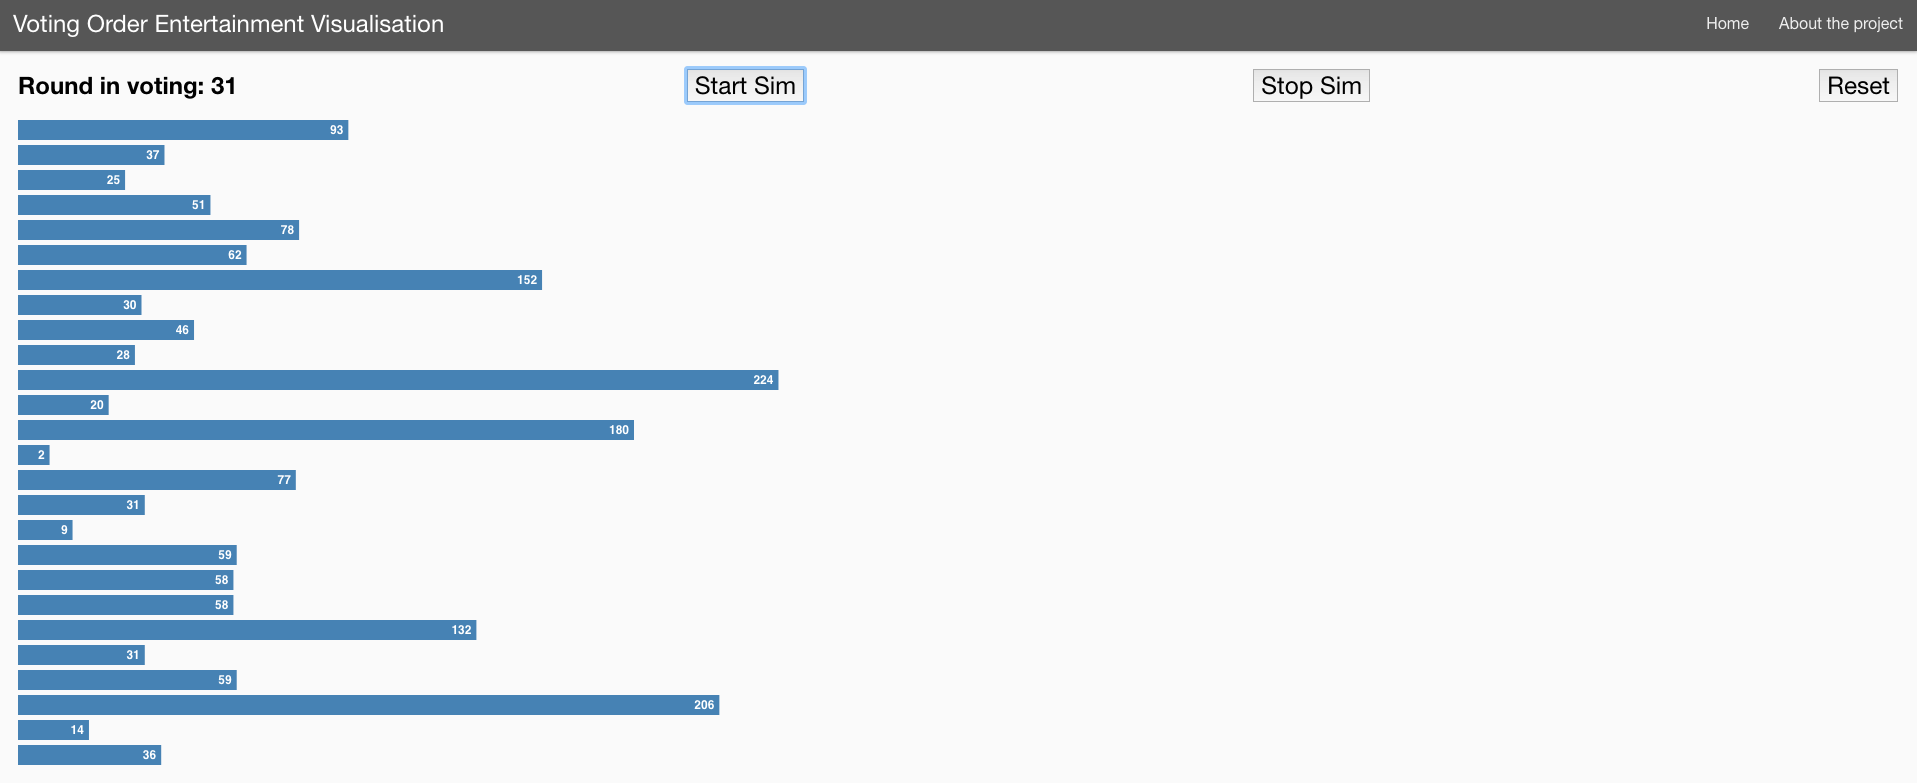
\includegraphics[width=17cm, height=10cm]{./visualisation}
\caption{Visualisation of solution to 2014 competition}
\label{visScreenshot}
\end{figure}

The application is a Node.js application that uses two main libraries for rendering the chart seen in Figure \ref{visScreenshot}. The first is \textit{d3.js} which is needed to scale the bars to the correct proportions as the scores are re-calculated. This uses the \textit{d3-scale} library\cite{d3} instead of using the whole of \textit{d3}. \textit{d3} could have theoretically taken care of updating of scores each round, however I was not extremely familiar with the way in which it updated state. Moreover for this project I wanted to produce something rather than getting stuck in the implementation details of learning a new library, and the more important part of this project was to produce solutions.

For this reason I turned to \textit{Preact.js}\cite{Preact}, which is a smaller and faster version of the currently very popular library \textit{React}\cite{React} from Facebook. I chose \textit{Preact}, as I have experience with React however I did not need the large number of functions that React provides and I needed the state changing to be fast, as there a calculations that need to be done from round to round. Moreover to speed up starting up the visualisation, the code is based on a \textit{Preact} example application.\cite{PreactBoilerplate}.

The visualisation is very simple, the user clicks a button to begin the competition voting and from there the scores are updated and shown on screen. A timer is used so that only one button press is needed to start the voting and from then on around every 1.5 seconds the new scores are shown, until the end of the competition. Moreover when a team cannot win, the colour of their bar is changed to grey, to help show who can still win. This provides anyone viewing the voting with a simple way to see how close certain teams are to each other and the current leader, and hence why the algorithms may have settled on this order. A further goal of producing this visualisation, which will be explained in Section \ref{FutureWork}, is using this visualisation as a tool for discovering new entertainment functions for this and other problems. 

As with the other code in this project I have attempted to make this as re-usable as possible. It takes the same types of inputs as the algorithms need, and any work to modify the code should only be purely cosmetic, such as changing names of \textit{voters} or \textit{participants}.

The visualisation code can be found in the \textit{visualisation} folder in the source code, along with explanations on how to run it to view it locally.

\section{Results and Evaluation}\label{Results}
% describe to what extent you achieved your goals
% describe how you demonstrate that the system works as intended (or not)
% include comprehensible summaries of the results of all critical test that were carried out
% should try to indicate how confident you are about whatever you have produced, and also suggest what tests would be required to gain further confidence
% describe the reasoning behind the tests to evaluate your results, what tests to execute, what results show and why to execute these tests
% include discussion of how you are designing your experiments to verify hypothesis of more scientifically oriented project
% e.g.. describe how you compare the performance of your algorithm to other algorithms to indicate better performance and why this is a sound approach. then summarise the results of the tests of experiments
% critically evaluate your results in the light of these tests, describing its strengths and weaknesses. ideas for improvement can be carried over into Future work.
% present a critical appraisal of the project as a whole, including why the programming language and methodology chosen were appropriate
\subsection{Overview of goals}
The main barrier to saying that this project achieved all of it's stated goals is the fact that the optimal solution is not know. The goals set out in Section \ref{Introduction} were:
\begin{enumerate}
\item a solution that delivers an entertaining competition when the votes are revealed
\item a way of describing entertainment mathematically
\item a way of visualising the competition as the votes are revealed.
\end{enumerate}

As it is the most important of the three goals, the goal of finding entertaining solutions is explored below in Section \ref{solutions} in more depth.

Describing the entertainment of a given voting order mathematically was explored theoretically in Section \ref{EntertainmentFunction} and their implementations in Section \ref{Imp-eFunctions}. In terms of success in achieving the goal, I think it was very successful. The main entertainment function (\textbf{refinedMaxMin}) provides a simple and elegant way of enumerating a concept that can be quite difficult to define. The functions not only define an entertaining solution mathematically, but they also allow them to be maximised or minimised easily, so in this regard they are also very accomplished in helping to achieve the first goal. A comparison between the two functions defined during the project and an explanation as to how they were tested against each other can be found in Section \ref{OtherTesting}. Moreover this will also provide more support as to why I believe this goal has been successfully reached.

It is more difficult to quantify if the goal of creating a way to visualise solutions has been met or not. In my opinion, the visualisation web application does a very good job of allowing another dimension of this project to be shown. The side of the project that the visualisation helps to shed light on, is essentially ignored by the algorithms and only generalised heavily in the entertainment functions. That is how real people would feel when viewing an "entertaining" solution. The visualisation provides a more visual style of feedback to the viewer. Furthermore it helps to justify the other goals without having to go into as much detail about the correctness of the algorithms or the entertainment functions, such as is done in this report.

All raw results can be found in the \textit{results} folder in the attached files.

\subsection{Solutions}\label{solutions}
This section will discuss both the general solutions found by all the algorithms and compare how they performed in finding solutions. Moreover the methodology for collecting and analysing these solutions will be explored. A table of the best and average solutions along with average times for each of the four algorithms can be found in table \ref{solutionsFound} and table \ref{timing} in the appendix respectfully. 

\subsubsection{Methodology}
% how got results and how analysed them
% how you designing your experiments to verify hypothesis of more scientifically oriented project
To find a set of solutions for each algorithm in order to analyse them, the first step was to do some repeated runs. To facilitate this some code was added to the main controller \textit{order.py} so that an optional command line parameter could be given which would repeat the running of the given algorithm how ever many times the user input. 

The general method was to run each of the algorithms lots of times and record the $\Phi$ and $\varepsilon$ values for that solution. From this we can be more confident about the performance of each algorithm and make some mathematical comparisons between them. To try and keep the experiment fair all the algorithms that take an initial solution were given the same one, that is the one given by the method \textit{getInitialSolution()} in \textit{support.py}.

An important point to recognise, before explaining the basic methodology, is that only testing of Greedy search and Simulated Annealing can be done in the exact same way, due to their similarities. Piecemeal and Brute force cannot be tested in the same way however the same idea of running them many times to collect many solutions still stands. Their methods are explained later on.

The experiments were designed to give each of the algorithms as much of a chance as possible to perform at their best. This meant that I attempted to keep the surrounding computation at a minimum so as not to add to the load on the CPU.

The experimental method for both Greedy search and Simulated Annealing are the same, apart from changing filenames. It begins with running a command in the terminal similar to that in Figure \ref{makeResults}.

\begin{figure}[H]
\caption{Running algorithms}
\label{makeResults}
\begin{verbatim}
>> python order.py simAnnealing 140 >> results/simAnnealingResults.txt
\end{verbatim}
\end{figure}
This command needs to be run in the same directory as the controller \textit{order.py} and the algorithm that is being run. In this example this command will run the Simulated Annealing algorithm 140 times and then send the output to a file called \textit{simulatedAnnealingResults.txt} in a \textit{results} subdirectory. 

The $>>$ part is a \textbf{bash} command that means append the output of the preceding command into the file after it. Append is used as it was necessary to run this code in smaller chunks to reach 1000 total runs. So as not to create a new file each time, we append from wherever we left off. Saving the output could have been achieved quite easily from within Python, however I felt that it was a sound idea to take the saving of the output away from Python as the terminal commands are usually faster and, in my opinion safer to use. They are also much more simple to write and have very little room for error. Moreover, when doing the timing experiments I wanted the least amount of overhead so that as little external time was spent on other computations that could accidentally leak into the times for the algorithms.

After doing this I was left with a set of files that contained both a $\Phi$ and an $\varepsilon$ value per line. These can be seen in the attached results files such as \textit{greedyResults.txt}. A snippet of this file is shown in Figure \ref{greedyResFile}.

\begin{figure}[H]
\caption{Snippet of Greedy results}
\label{greedyResFile}
\begin{verbatim}
...
(['Russia', 'Portugal', 'Ukraine', 'Poland', 'Sweden', 'Switzerland', 'Montenegro',
'Romania', 'San Marino', 'Italy', 'Latvia', 'Malta', 'The Netherlands', 'Slovenia', 
'FYR Macedonia', 'Ireland', 'Hungary', 'Iceland', 'United Kingdom', 'Lithuania', 
'Georgia', 'Norway', 'Germany', 'Greece', 'Israel', 'Spain', 'Armenia', 'Estonia', 
'Austria', 'France', 'Finland', 'Belgium', 'Denmark', 'Albania', 'Belarus', 'Moldova', 
'Azerbaijan'], 3409)
(['Italy', 'Russia', 'Ukraine', 'San Marino', 'Latvia', 'Norway', 'Israel', 'Belarus', 
'Slovenia', 'United Kingdom', 'Poland', 'Portugal', 'Romania', 'Georgia', 'Albania', 
'Denmark', 'Montenegro', 'Lithuania', 'Switzerland', 'Austria', 'The Netherlands', 
'Germany', 'Azerbaijan', 'Armenia', 'Ireland', 'Spain', 'Greece', 'Moldova', 
'Hungary', 'Finland', 'Belgium', 'Iceland', 'FYR Macedonia', 'Sweden', 'France', 
'Malta', 'Estonia'], 3298)
...
\end{verbatim}
\end{figure}

Although the $\Phi$ are very interesting in their own right, for them to make more sense and the find the best, it was necessary to extract the $\varepsilon$ values from this file so that some analysis could be done. To do this I used \textit{ack}\cite{ack}, which is a tool that allows for searching of plaintext files for lines that match a given regular expression. This allowed me to extract just the scores from the files like \textit{greedyResults.txt} and then send them to a file such as \textit{greedyScores.txt}\footnote{\textit{greedyScores.txt} can be found in the attached code and results.}. The command for this is shown in Figure \ref{ackCommand}.

\begin{figure}[H]
\caption{Extracting scores from results file}
\label{ackCommand}
\begin{verbatim}
>> ack -o "(?<=,\s)\d{4}(?=\))" algorithmResults.txt > algorithmScores.txt
\end{verbatim}
\end{figure}

The \textit{ack} tool uses Perl regular expressions for matching the given expression. In this case the regular expression is very simple but looks complex. The \textbackslash d\{4\} part matches 4 of any digit. The parts before in brackets is a \textit{positive lookbehind} and after in brackets is a \textit{positive lookahead}. These match something before or after the digits but do not keep them in the output; and are used to find a comma and a space before, and the final bracket after the score. The \textit{-o} part is a flag that is used to only print whatever is matched, otherwise the whole line where a match was found would be printed and there would be no difference between the results and score files. Once again we use the \textbf{bash} commands to send the output to a file, however this time we do not append, but create the file and write to it immediately.

After doing this we have files that contain 1000 $\varepsilon$ values, which can then easily be copied into Microsoft Excel for analysis.

When running the two search algorithms there are some setup values that are needed. The main one is \textit{num\_iterations}, which both Simulated Annealing and Greedy Search use. To try and keep the tests as close to each other the same value was used ($num\_iterations = 500$).

Specific to Simulated Annealing's case there are some more input values that are needed, and they were discussed in Section \ref{Algorithms} in the pseudocode. The final values are shown in Table \ref{coolingValues} in the appendix. To reach these values I took into account more general wisdom for each one as well as trying to apply more problem specific knowledge to reach the values that give the best solutions. Furthermore, the time taken to find a solution could be heavily effected by the values so a balance was struck so that the algorithm did not take too long, but also produced consistently good $\varepsilon$ values.

% method of finding piecemeal different - try every first country
The methodology for the Piecemeal algorithm was slightly different. This is due to the fact that given the same first choice the $\varepsilon$ value will always be the same. The problem of which \textit{voter} should be first, was brought up in Section \ref{Algorithms}. It was decided to try and find the best solution by trying all the possible first choices and saving them all. This takes away the random element but still allows the algorithm to return it's best possible solution.

To do this it was necessary to wrap the Piecemeal code as shown in Figure \ref{piecemealCode} inside a \textit{for} loop and instead of hard-coding the first element on lines 10, 11 and 12, using the index from the loop.

Once again to extract the scores I used the same \textit{ack} command from Figure \ref{ackCommand} to find the scores and send them to a file.

% methodology of finding brute force
As the Brute force algorithm can not be run in the same way as the other three, a different method was devised to test it. The method was to leave it running for 1 hour. This is a fair time to run it for, as will be discussed in the timing part of this section. The other algorithms produce solutions consistently in under 20 seconds. As before the experimental conditions were as similar as possible to the other tests. In this case all the solutions found were saved and the best solution found was the last one found after 1 hour.


\subsubsection{Solutions found}
% Pick out interesting values of solutions and talk about which algorithms are better than each other
% indicate how confident you are about solutions, and also suggest what tests would be required to gain further confidence
The best $\Phi$ for the 2014 Eurovision was found by Simulated Annealing with a $\varepsilon$ value of \textbf{2554} (using \textbf{refinedMaxMin}). Although is it difficult to say with certainty if this ordering is the \textit{globally} optimal solution for the 2014 Eurovision competition, I believe that we can say with a high degree of confidence that this solution is at least close to optimal. This suggests that in terms of achieving the goal of finding a solution that delivers an entertaining competition, this project has been successful. This is true because even if the best solution found is not the \textit{"optimal"} one, it is still very much an \textit{"entertaining"} one.

\begin{figure}[H]
\caption{Best solution}
\label{bestSolution}
\begin{verbatim}
['Belarus', 'Albania', 'Poland', 'United Kingdom', 'Montenegro', 'Armenia', 'Malta', 
'Russia', 'Azerbaijan', 'Germany', 'San Marino', 'Italy', 'FYR Macedonia', 
'Moldova', 'Estonia', 'Austria', 'Romania', 'Switzerland', 'Ukraine', 'Latvia', 
'Denmark', 'Georgia', 'Hungary', 'Finland', 'Ireland', 'Norway', 'Greece', 
'Spain', 'Israel', 'Portugal', 'Lithuania', 'France', 'Belgium', 'Iceland', 
'Sweden', 'Slovenia', 'The Netherlands']
\end{verbatim}
\end{figure}

To try and verify if this was the most optimal solution that could be found, this $\Phi$ was given to both Greedy and Simulated Annealing as the initial solution, and they were run around 10 times. They both returned this same solution, which gives good confidence that this is the best possible $\Phi$.

Table \ref{solutionsFound} in the appendix shows some of the other interesting $\varepsilon$ values found for all the algorithms used. The $\Phi$ corresponding to those values is not shown as they are very long, however finding them is a case of searching the results file for the $\varepsilon$ value as they are saved together.

Figure \ref{eScreenshot} shows Simulated Annealing, Greedy and Piecemeal with their minimum, average and maximum $\varepsilon$ values so they can be compared.

\begin{figure}[H]
\centering
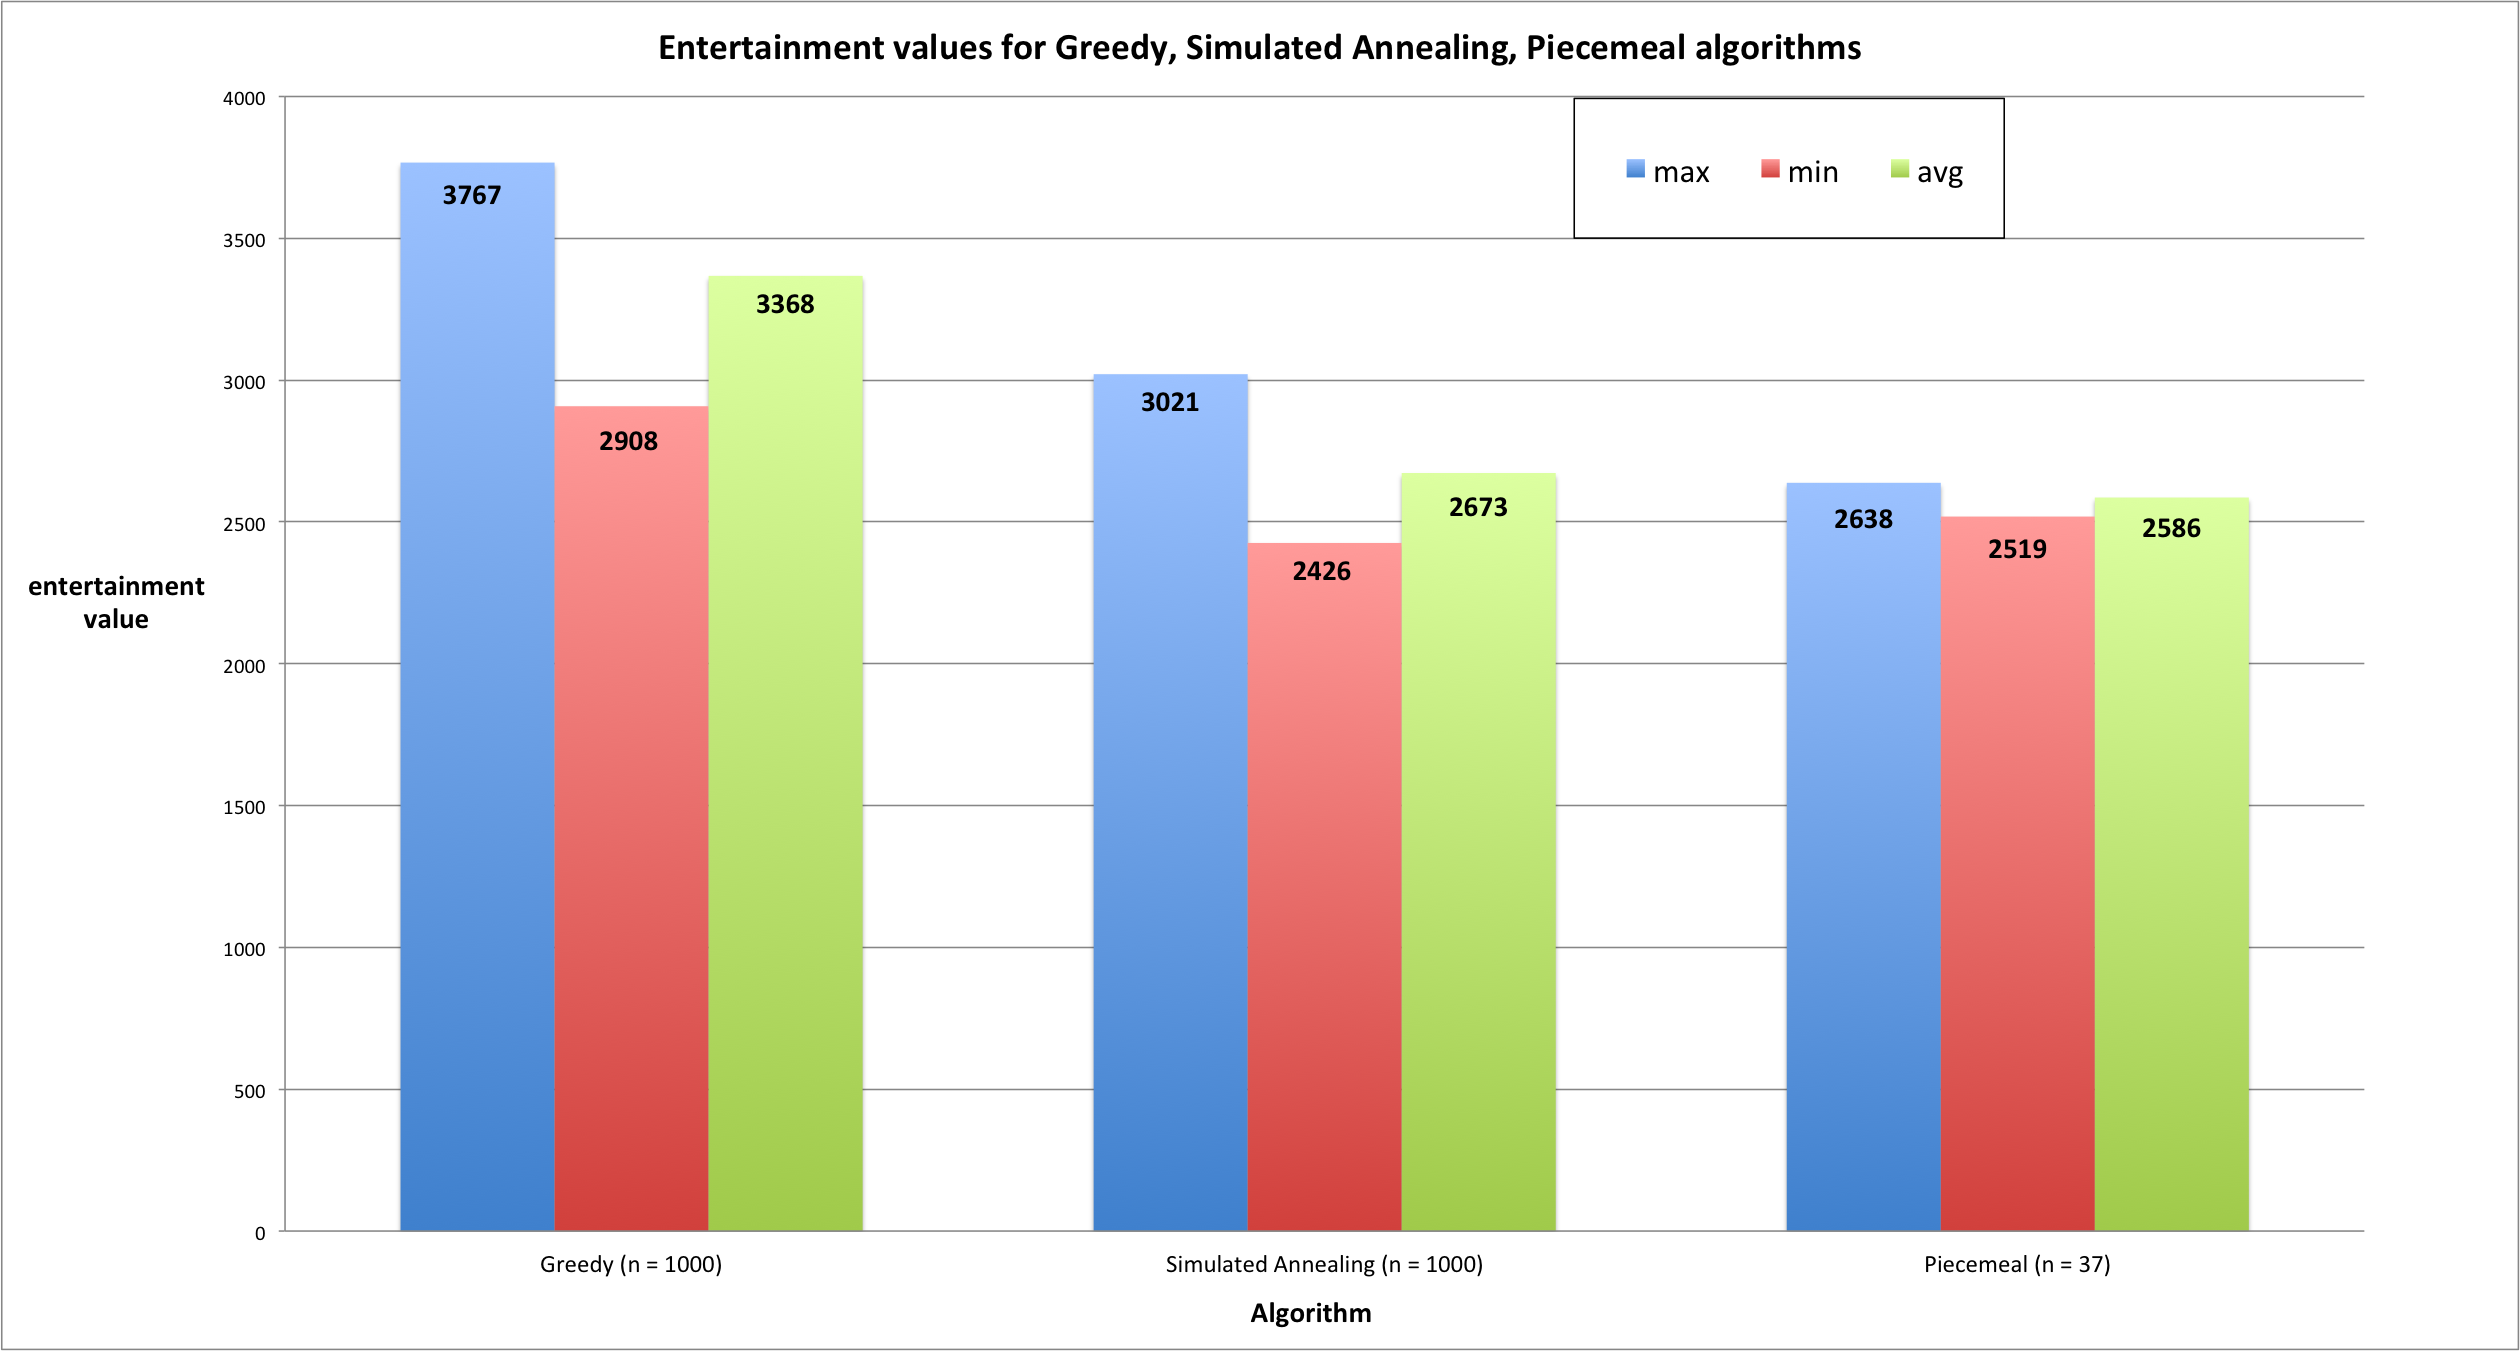
\includegraphics[width=18cm, height=11cm]{./entertainmentValues}
\caption{Chart of $\varepsilon$ values found by Greedy, Simulated Annealing and Piecemeal}
\label{eScreenshot}
\end{figure}

In terms of comparing the algorithms the first point is that Simulated Annealing is the best algorithm as it found the best $\varepsilon$ value and hence solution as discussed above. This is in terms of $\varepsilon$ value found only, and not with respect to any other measure of quality such as speed. How they compare in other regards is discussed in Section \ref{OtherTesting}.

The Greedy algorithm does not perform particularly well as it's average $\varepsilon$ is much higher than the other two. Moreover the best $\Phi$ it found has a $\varepsilon$ value of \textbf{3196}, which is about 150 worse than the worst $\varepsilon$ value that Simulated Annealing found. The large range of values as seen from the large difference between the max and min means that Greedy is not a consistent algorithm when given consistent input, as in this problem. This backs up the idea that lead to the development and use of Simulated Annealing and Piecemeal for this project as Greedy did not find very optimal solutions. If the results produced by Greedy were better, then there would have been little gained from the rest of the project. 

One interesting point that is not shown in Figure \ref{eScreenshot} is that if we use a solution given by the Piecemeal algorithm as the initial solution, then Greedy \textit{can} perform as well as Simulated Annealing (given the same initial solution as before). This increase in quality when given an already good $\Phi$ is shared by Simulated Annealing. This leads to the conclusion that Greedy is getting stuck in local minima and as it has no means of escaping them, returns the best $\Phi$ that it has.

The Piecemeal method was a major success for this problem, especially as it is not a general algorithm like the others, which have been proven and tested on many problems. Referring to Figure \ref{eScreenshot} the chart shows that the Piecemeal method held it's own against a much more complex and established algorithm in Simulated Annealing. The lowest $\varepsilon$ value that it found was \textbf{2690} which is only 17 worse than the globally best solution found. Moreover as can be seen from the range of values, this method is consistent in returning good solutions, when varying the first \textit{voter}. This may be because the only difference between the attempts is the first voter, however that is the only part that is changeable between runs. As the averages of both Simulated Annealing and Piecemeal are very similar we can say that Piecemeal is almost as good as Simulated Annealing at finding consistently good solutions.

% talk about future work on testing solutions found against people

\subsection{Testing}\label{OtherTesting}
% describe the reasoning behind the tests to evaluate your results, what tests to execute, what results show and why to execute these tests
The entertainment of a solution is not the only thing that gives it value. This is why some other testing was undertaken to try and give a more well rounded picture of how well the algorithms performed on this problem. Taking all the tests executed together gives a higher level of confidence in the results as there is more experimental data that can then be leaned on when evaluating the project as a whole and when making future decision about algorithm choice for other, similar, problems.

\subsubsection{Timing and Big-O Complexity}
As well as producing results that maximise entertainment, it is necessary for the algorithm to do so in a reasonable time. Table \ref{timing} contains some results for timing of the algorithms.

The methodology for analysing the timing was to run each of the algorithms 100 times each and have timing set to show how long it took for the function that runs the algorithm to finish. The timing is done using the \textit{timeit}\cite{PythonTimeit} library in Python, which purports to take care of many common pitfalls when timing code. It should be advised that these timing values are not necessarily the best, which is why they are averaged over 100 runs.

\begin{figure}[H]
\caption{How to time the algorithms using Python}
\label{timingCode}
\begin{verbatim}
from timeit import default_timer as timer
...
start = timer()
print(gs.greedySearch(SCOREBOARD, PERFORMING_COUNTRIES, VOTING_COUNTRIES, 12))
end = timer()
print('algorithm took: ', end - start)
\end{verbatim}
\end{figure}

After sending those results into a file using the same method as for the solutions, I again used \textit{ack} to extract the times and send them to a timing file. An example of the command to do this is shown in Figure \ref{timingAck}.

\begin{figure}[H]
\caption{Extracting times from a results file}
\label{timingAck}
\begin{verbatim}
ack -o "(?<=\('algorithm took: ',\s)\d+.\d+" greedyTiming.txt >> greedyTiming.txt
\end{verbatim}
\end{figure}

This varies slightly from the \textit{ack} command for the solutions, as it must look for values with decimals, which it does by looking for any number of digits followed by a decimal place, followed by any number of digits.

From there I copied the values into the attached \textit{Results} excel file. Direct comparison is quite difficult to visualise as there is a huge difference in the running times of the main algorithms. Due to Brute force's special situation no results are collected for it.

The first thing to notice is that Simulated Annealing is the slowest, taking an average of almost $13$ seconds to return a solution. Greedy on the other hand is very quick taking on average half a second to return a solution. Finally by far the fastest is Piecemeal which on average takes around $8$ milliseconds to return a solution.

So compared to Simulated Annealing, Greedy is $\approx 25$ times faster $(4 s.f)$ and Piecemeal is $\approx 1606$ times faster $(4 s.f)$. Moreover Piecemeal is $\approx 63$ times faster than Greedy.

When these timing results are taken with the $\varepsilon$ values that each algorithm found, we can make judgments as to why some algorithms are better than others. For example, even though Greedy returns solutions in less than a second the quality of those solutions are not very good. This is especially obvious when comparing Greedy to Piecemeal as the later is faster, and also returns solutions with a better $\varepsilon$ value. This leads to the conclusion that Piecemeal should always be used over Greedy. When looking at Simulated Annealing, a large point in it's favour is the fact that it found the globally best solution. However a major point to it's detriment is the fact that it does so over $1600$ times slower than Piecemeal, which finds a near to best solution. When deciding between Piecemeal and Simulated Annealing, a value judgment would have to be made in regards to what is more important speed or finding the best result. If speed is the main factor, and a close to best solution is good enough then Piecemeal is the obvious choice. If waiting $\approx 15$ seconds for a solution but having a good chance of finding the best is the overriding goal then Simulated Annealing is the better choice.

Another inherent part of the algorithms is their Big-O complexity. This describes how the algorithms will scale to different size inputs. Explanation of each algorithms complexity in turn can be found in Section \ref{Algorithms} and Table \ref{bigO} summarises them. The complexity has a large effect of the runtime of the algorithms so it is useful to look at the theorised complexities and see if they compare to experimental runtimes. Although the algorithms have not been run against various sizes of input it can still be interesting to compare between the algorithms.

For example, following the complexities in Table \ref{bigO}, Piecemeal should be the fastest followed by Greedy and then Simulated Annealing, with Brute force taking a computationally infeasible time. This theory is backed up by the timing results that suggest the same. So in this way running the timing experiments is useful for proving the  hypotheses explained in Section \ref{AlgorithmDesigns}, as well as helping with decision making.

\subsubsection{Partial and Full $\varepsilon$ calculation}
It was theorised that, as well as producing more realistic and exciting solutions, the partial calculation method described in Section \ref{Imp-Ewrappers} also reduces computation time for any algorithm that uses it.

To find out if that is true first it was necessary to run both of the functions \textbf{getEntertainment} (which uses full calculation each time) and \textbf{offsetGetEntertainment} (which uses partial calculation) side by side. When doing this the actual final solutions that were found were discarded as the extra overhead of doing 2 calculations of the same entertainment value could have adversely affected the results. The timing method was the same as used for the general algorithms (see Figure \ref{timingCode}).

To get the results, the Greedy algorithm was run and its output saved to a file as before. To distinguish the times, the full calculation was output with "full" before it and the partial time with "reduced" before it. Once again an \textit{ack} command similar to Figure \ref{timingAck} was used to extract the times and save them to another file specific for either reduced or full times. This produced 10,000 values for each of the methods which were then analysed in Excel.

Figure \ref{f_recalcComparison} shows the average time over those 10,000 iterations. The actual time taken is not the interesting part, more interesting is the fact that the reduced method takes around half the time. This result supports the hypothesis above in that it shows that the computation time for the reduced calculation is indeed lower. This also means that the computation time for any algorithm using it is also going to be lower. A further point that speaks to why the reduced method is better is that it is used many, many times during the course of finding a solution to this problem, so any saving in terms of computation time will be heavily felt by the overall time to reach a solution.

One drawback of this method is that it does not always guarantee the same reduction in time over the full method. As was described in Section \ref{Neighbours}, the amount of calculations needed is dependent on where in the order the swaps take place. The number of calculations range from being at worst the same as the full method to being only around 50 total calculations. If the reduced method must calculate the same or nearly the same number as the full method, it is likely that the time reductions will have been unfortunately lost due to setup overhead in the function.

\begin{figure}[H]
\centering
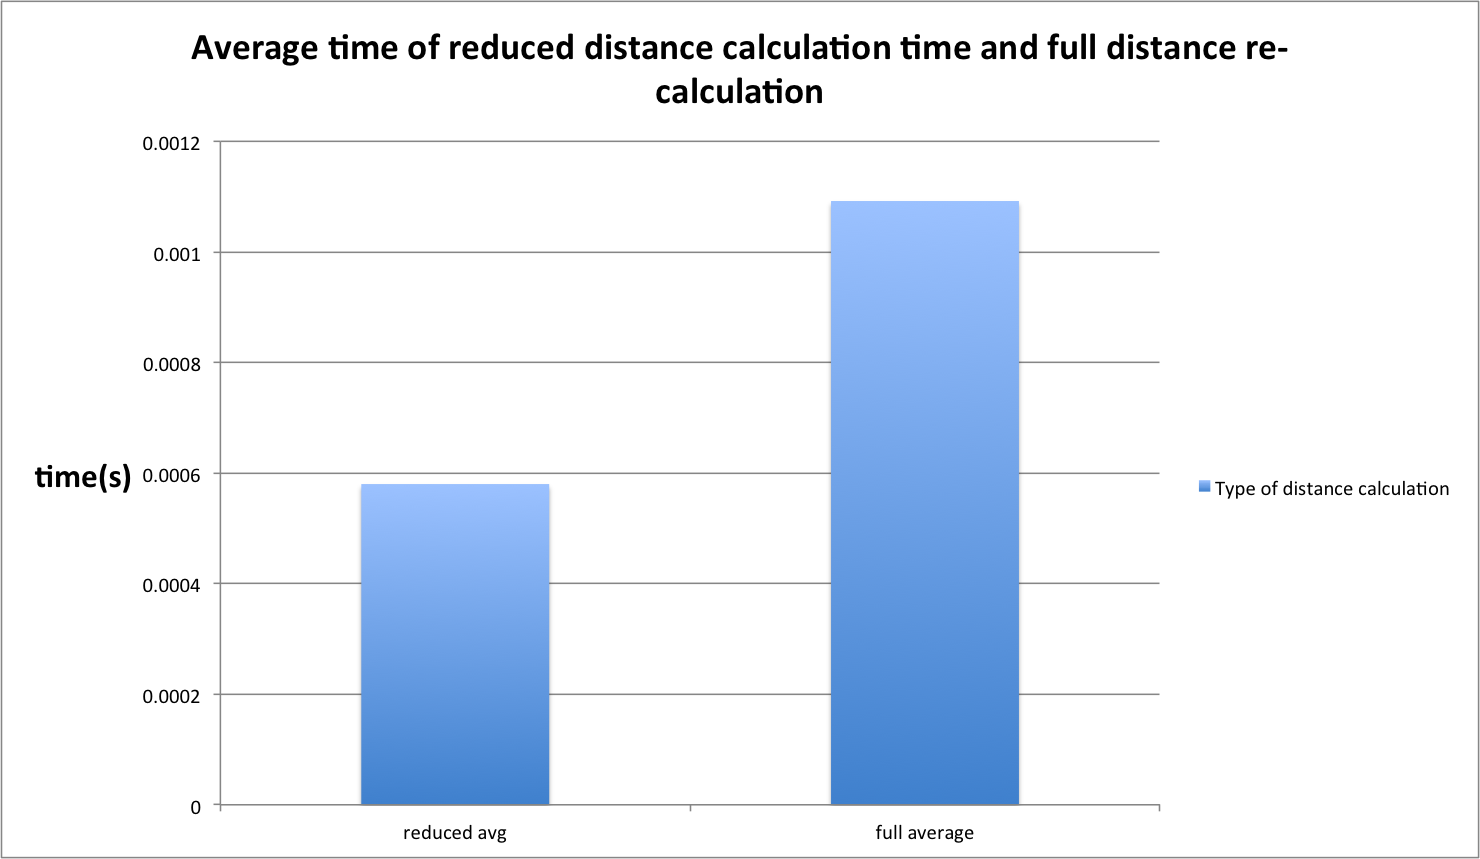
\includegraphics[width=18cm, height=10cm]{../code/misc/reducedvsFullDistanceCalc}
\caption{Average time taken to perform full and partial $\varepsilon$ calculation on the same solution}
\label{f_recalcComparison}
\end{figure}

To make sure that the reduced method was indeed correctly calculating the $\varepsilon$ value it was decided to run them side by side and compare their results. This could quite easily be done as the testing setup necessary to log the times required that they both be run every time. The test was essentially to equate the two outputs after they were run and to print "true" or "false" if they were the same or different. This adds to the confidence in the method as it was quite easy to return to test that at any time after any major changes to the algorithms or main support methods.

\subsubsection{maxMin and refinedMaxMin}
The theoretical reasons why the \textbf{refinedMaxMin} method is better, such as giving a more real picture of entertainment, have been discussed. To try and find some evidence for this, the  minimum values that each method returned were found. To do this the same method as for the full and partial $\varepsilon$ calculations test was followed. That was to run both methods side by side and return the minimum values that were found in two lists which could then be analysed.

The effect that the refined method has on the minimum value that is used in Equation 1, is shown in Figure \ref{f_maxminDif}. The graph shows the minimum scores that are returned by the two methods as green and blue points, as well as the difference between the two values (red line and red numbers) over a single typical competition. From this graph it can be seen that the \textbf{maxMin} method stays relatively low as in this competition the lowest score at the end was only 2 points. On the other hand, the \textbf{refinedMaxMin} method diverges at around round 22. This is when it can start ruling out \textit{performers} from winning the overall crown. By the last few rounds the difference is quite large as there are only a few countries that could still win; so only their scores are being taken into account for entertainment.

\begin{figure}[H]
\centering
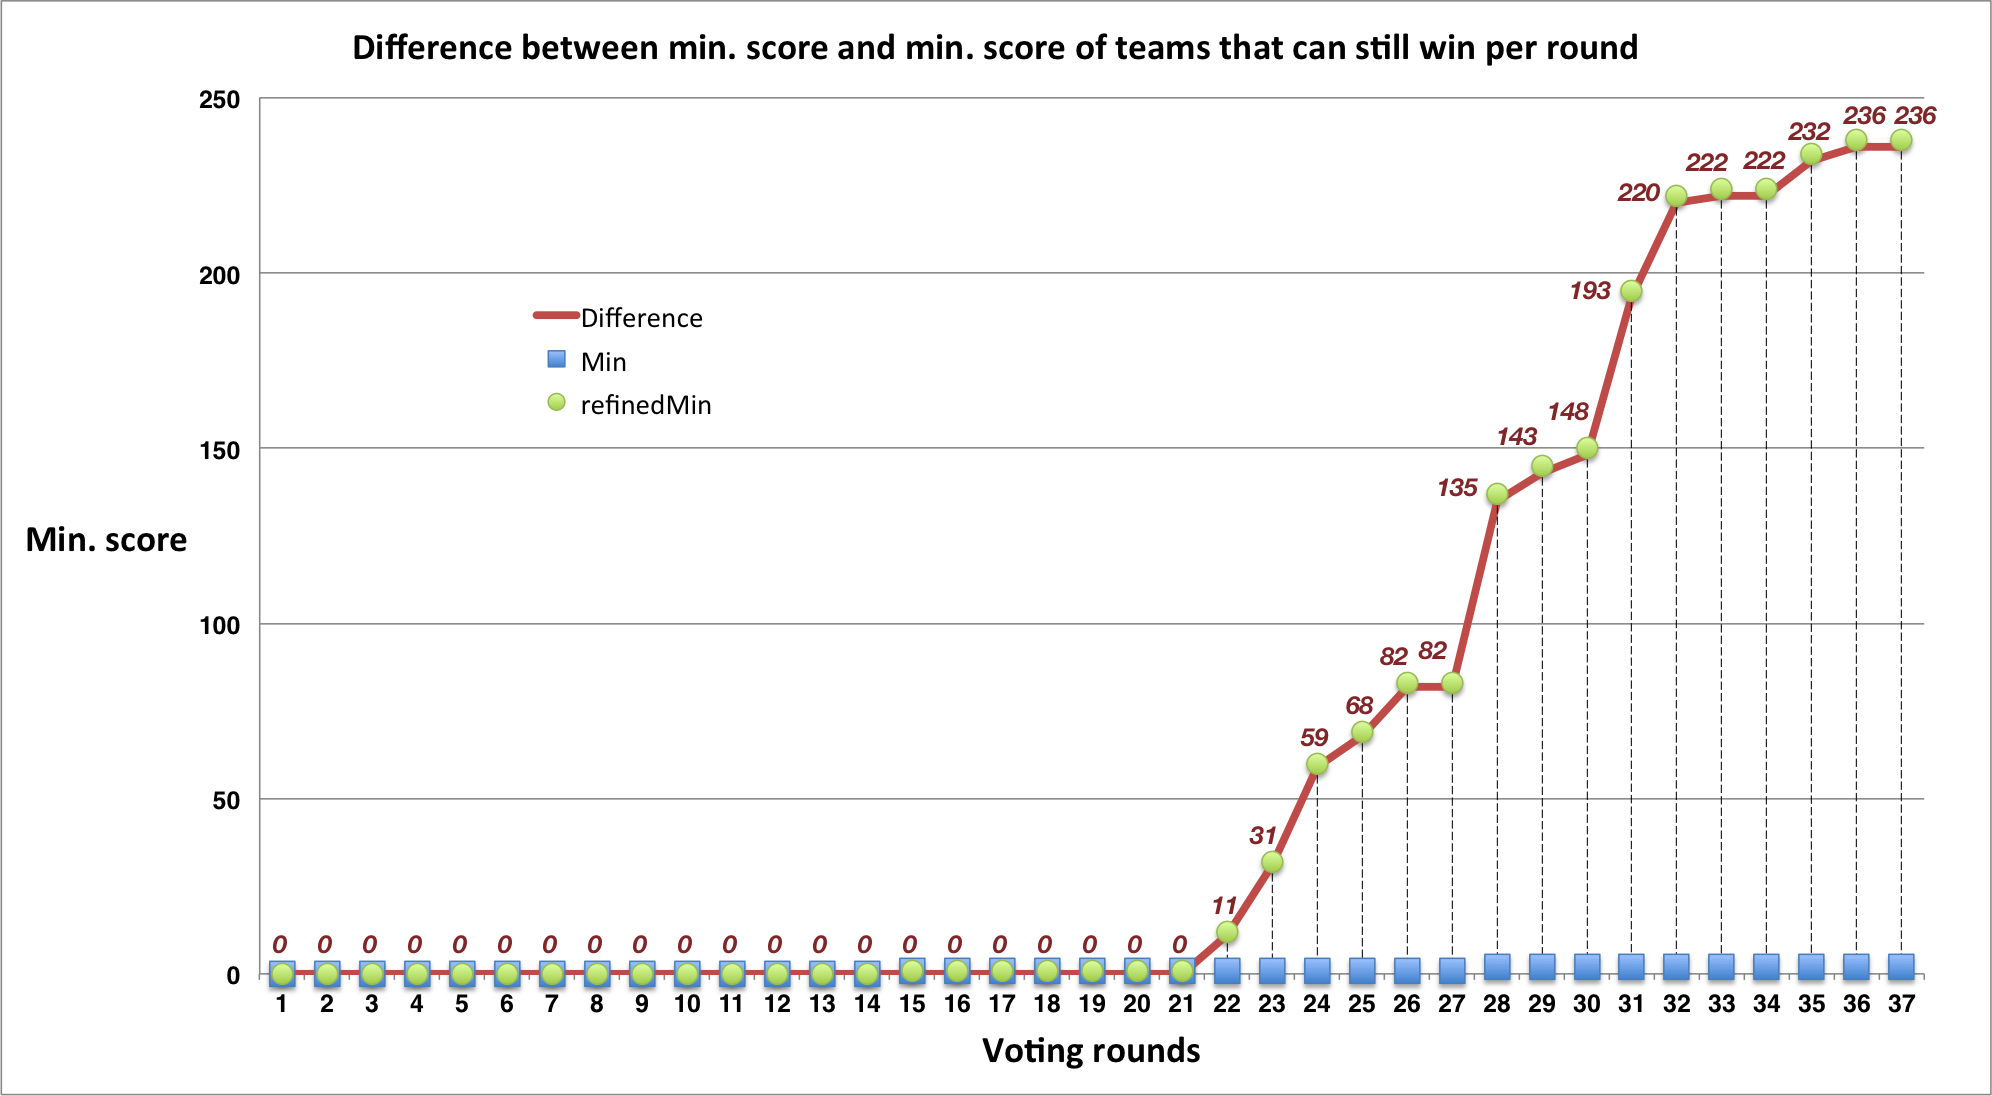
\includegraphics[width=18cm, height=10cm]{../code/misc/difference_MinvsRefinedMin}
\caption{Difference between min value found for MaxMin method and RefinedMaxMin}
\label{f_maxminDif}
\end{figure}

This chart helps to explain why the idea of removing teams that can no longer win from the calculation can aid in achieving better solutions. The \textbf{maxMin} method only ever really returns a value less than 5, which corresponds to the country currently in last place. It is easy to see that nearer the end of the competition those countries are not adding anything to the entertainment of who will win as their scores are near 0. On the other hand, the \textbf{refinedMaxMin} method begins to prune the losing countries, and by the end is only looking at a small group of countries that can still win.

Another point to take into account is the complexities that these methods have and how they can affect the choice to use them. Table \ref{maxMinComp} in Section \ref{Imp-eFunctions} shows the complexities of the two methods. Taking this with the results from Figure \ref{f_maxminDif}, even though the complexity of the refined method is slightly higher, the value that it adds means that the trade-off is worth it in my opinion.

\subsubsection{Comparing solutions}
% order_diff.py
Throughout the project the same problem kept appearing while trying to compare the intermediate or final solutions. For my piece of mind I wanted to know if similar $\Phi$ were giving similar $\varepsilon$ values and have a quick way to compare two $\Phi$ without having to manually look at country names and compare in what position they were. Moreover having a way to almost immediately know if two orders were the same was very helpful as separating orders based solely on their $\varepsilon$ values was not good enough as the values could be shared by vastly different orders. It was also helpful to find a way to see if there were common groupings or positioning of \textit{voters} in different solutions.

To solve this problem a quick and simple Python script was written which can be see in Figure \ref{orderDiff}. In the full source code that is attached, the code differs slightly as this code is not meant for use during the running of any algorithms so the file has manually hard-coded values for the orders, $order1$ and $order2$.

The idea behind it is very simple, if there are two orders that are different, sum up by how many places the same \textit{voters} are separated in each. This occurs on line 4, where the $dist$ variable is the total sum of the difference between the indexes of the same \textit{voter}. By using the $abs()$ method from the Python standard library it was possible to not worry about which index was higher and hence keep the code simple.

\begin{figure}[H]
\caption{Finding the difference between two orders}
\label{orderDiff}
\begin{lstlisting}
dist = 0
for country in (order1):
  index1, index2 = order1.index(country), order2.index(country)
  dist = dist + abs(index1 - index2)
print(dist)
\end{lstlisting}
\end{figure}

\subsubsection{Unit tests}
As the main algorithms do not have repeatable behaviour, due to the fact that they rely on a random step to help pick solutions to look at, it is not possible to unit test them without defeating the purpose of unit testing. There are however some functions that can be unit tested. The file \textit{orderTest.py} contains these tests. The methods that are tested are \textbf{getAdjacentNeighbour}, \textbf{getNeighbour}, and \textbf{refinedMaxMin}.

The tests themselves should be fairly self explanatory they call the function with set inputs and assert that the output from that function matches some value or set of values.

Although these tests are not strictly necessary for the completeness of the project, they help to provide another level of confidence along with the in-place testing described in this section. The tests are not the most comprehensive and only really test the simple working of the methods. The main reason for the lack of unit testing is that this project does not have an already known result, which is something that unit tests require. 

\subsection{Critical Evaluation}\label{Eval}
% talk about Python as a choice
% critically evaluate your results in the light of these tests, describing its strengths and weaknesses. ideas for improvement can be carried over into Future work.
%  -- running using same initial solution each time -- randomise?
% present a critical appraisal of the project as a whole, including why the programming language and methodology chosen were appropriate
The main strength of the results lie in the analysis and the methodology for collecting and analysing them. These results, and the tests that were run to verify them, point to the fact that the project's results are correct and that they can hold up to scrutiny. The analysis has also shown that the results are significant in terms of reaching the goals set out at the start of the project. 

On the other hand, a weakness of the results is the small amount of testing of the overall system as it runs. This could be seen as problematic as there are many moving parts that allow an algorithm to be run and produce solutions. Although some of these have been mitigated through other testing, it is always possible that there are still mistakes. Furthermore even though the manual testing attempted to reduce the likelihood of any problems showing up, as always with manual testing, human error can cause problems to be missed.

Another strength of this project was the scientifically-minded method in which each stage was undertaken. Each decision, such as writing a new algorithm or method, was based on intermediate experiments and experimental data. By doing this at every stage throughout the project, a higher level of confidence is gained in the final results, as there are explainable reasons for all the decisions made, and data to support them.

One important point to evaluate is the use of Python as the programming language for this project. Overall the biggest strength that Python brought to the project was it's ease of use. This manifested itself not only in the actual writing of code for the project, but also the supporting overheads that any programming language brings with it. For example, the good quality and reliable standard libraries helped to reduce workload for the more complex parts of the code. Moreover running the algorithms was simple, allowing manual testing to be done with little hassle, where using another language would have added extra setup and time. 

A common weakness that is levelled at Python is it's lack of complex data structures and types. For this project, this was not a problem as although the algorithms may be complex, the data structures needed were not anything more complex than an array (list in Python). Having experience with Python also helped to mitigate any problems before they cropped up, such as stopping the global amendment of lists by copying them instead of passing the same list between functions. This can be seen in many places in the code as there is heavy use of code similar to $newList = oldList[:]$, which sets $newList$ equal to a copy of $oldList$ instead of setting it equal to $oldList$ itself. In other languages such as Java this would not be problem, however it would likely bring its own quirks. Overall it is fair to say that Python performed extremely well for this project.

\section{Future Work}\label{FutureWork}
% expressing unrealistic ideas, including what you would have liked to have done if only you had not run out of time
% provide a good starting point for someone else to continue the work which you have begun
The first and most obvious point for future work would be finding out if the best $\Phi$ found is globally optimal and if it is not, then finding the globally optimal solution. Although the Brute force method had to be abandoned due to it's computational infeasibility, it may be possible that by using heuristics with the Brute force algorithm to cut down the search space, the globally optimal solution could be found.

Another thought for future work relates to testing the entertaining solutions that were produced, using people. This would be taking a more Psychological or Sociological approach to the project instead of just mathematical. This testing could take place as a sort of mock version of Eurovision where different groups of spectators are shown the voting in different orders and then must rank them in terms of excitement and entertainment. Moreover, by using questionnaires of those who undertake the study, it could be possible to uncover new entertainment functions that were as yet unrealised.

New functions could also be developed separately. In this project we have concentrated only on who can win the competition, however entertainment will contain many more parts. For example, maximising the entertainment for as many spectators as possible who are rooting for each country, possibly taking into account population and engagement of the viewers. Other functions could be ones that maximise those who can reach a certain position, in competitions that involve multiple prizes such as finishing above a certain place. Another would be for competitions with relegations, keeping as many participants in the fight to stay up for as long as possible.

Specifically related to the \textbf{refinedMaxMin} method, some future work would be to improve the upper bound score calculation, as it currently does not take into account the possibility that teams may have to vote for themselves and hence not be able to receive 12 points in \textit{every} following round. This improvement should be as simple as tracking who has voted and who is yet to vote and remove 12 points if the current team is yet to vote.

A final piece of future work would be to try and optimise the code for performance. This would take a little more of a deeper understanding and investigation into Python as although I was experienced in using it, never for high performance code. Moreover there are likely places in the code that are not optimised as I prioritised getting correct results over the code being the most performant.

\section{Conclusions}\label{Conclusions}
% summary of the aims of the project and a restatement of the main results, i.e. what has been learnt and achieved
% an effective set of conclusions should not introduce new material. Instead it should briefly draw out, summarise, combined and reiterate the main points that have been made in the body of the project report and present opinions based on them
The main aims of the project were to find an ordering of voters that maximises entertainment, to develop some functions that could codify entertainment mathematically and to produce a way of visualising an ordering.

In terms of these goals, I believe all of them have been achieved to a high degree of quality. The algorithms produced found a solution to the problem that successfully maximised the entertainment. The functions that were produced to describe entertainment were very successful in taking the intuitive feelings of entertainment and turning them into mathematical functions. Finally the visualisation produced can clearly be shown to aid in the understanding of what makes these good solutions better than the bad ones. Moreover the experimental results outlined in Section \ref{Results} help to support the idea that these goals have been achieved.

From this report it should be possible to see that novel implementations for use in these types of problems have been produced. Moreover these novel methods have been properly backed up with experimental results in order that their correctness is not in doubt. Also the upmost has been done so that this project does not stand alone with no use for any future work in this area. I think it is fair to say that this project could lay some groundwork for solving more problems from this specific area of optimisation problems, albeit with some additions or modifications.

As can be seen from the context of this project in Section \ref{Project Context}, there has not been a large amount of research into maximising entertainment, especially in the field of Computer Science. This means that although this project began with concrete goals, there was no real context to give an insight into how to best approach the problem, or how simple or complex finding a solution would be. In that respect, achieving the stated goals shows the overall success of the project. 

Furthermore it can be said that due to the lack of current research, this project has added a good amount to the research area of optimising competitions for entertainment, by providing a good base for other similar projects, and some useful insights into how to approach these types of problems.

\section{Reflection on Learning}\label{Reflection}
% identify the impact of what we have done on the assumptions, concepts and ideas we used to make decisions about our work
% try to identify the characteristics of the problem that has been addressed , and consider whether assumptions of decisions about the relevant approach to solving the problem had been appropriate, in order to make a better decision in relation to problems that might be encountered in the future.

I think that by assuming that the problem we were undertaking would be complex, we avoided a range of problems that could have arisen. This way of approaching problems (that have an unknown solution) is extremely transferable. From this project I have learnt that not underestimating the complexity of problems will also mean that you are more open to pivoting when problems do arise. Moreover the idea to continually look at data and use that to make decisions, could only be achieved if the problems complexity is thoroughly thought through before starting the project.

Giving myself the freedom to change tact based on changing results also relied on having a solid plan that was still flexible. For this plan to be useful whilst also following the learning from above, it needed to be sufficiently detailed so that I was never lost, but also allow me the freedom to swap tasks around depending on how things were going. In that respect I learnt a lot about planning complex projects in an Agile fashion. I think having the ability to react to changing contexts and information is a valuable skill that this project has given me.

On the point of planning in this project, another new skill gained is to be very industrious with my time. Even though throughout I had the aid of my supervisor, how I spent the majority of the time had to be decided by me. Especially for such a long project with many parts to it, this was complicated. I believe that I gained a deeper understanding of managing my time for a large and complex problem by splitting it up and attacking specific areas. For example by breaking the project up into the three sections (Entertainment functions, optimisation algorithms and visualisation) in the Initial Plan and then looking at those as the major milestones, it took some pressure off me. I could happily change details of what tasks I needed to complete next and still reach that larger milestones. This again is an extremely useful skill to have gained by virtue of this project.

The work plan is attached in the appendix, and shows a fully updated version of the Initial Plan. The main overarching point is that for many of the tasks the \textit{plan start} and \textit{actual start} differ. As discussed this did not really adversely affect the project, as it was possible to bring forward the implementation of the visualisation and then return to implementing new algorithms easily. I learnt a lot about flexible planning by having this type of plan to refer to when changes were necessary.

Another major skill I have learnt from this project, is to always be sceptical of results until after a deeper analysis. On a couple of occasions during the project I was faced with intermediate results that did not match up with my hypothesis. When faced with this data, I did not immediately throw away the hypothesis and formulate a new one, but I used that initial data to start a deeper investigation. From this I learnt that in problems such as this, there can be hidden phenomena that do not necessarily match up with your first thoughts. These hidden problems can be causing side affects, that are observable, however the problems actually lie deeper. 

For example after initially developing the Piecemeal algorithm it was producing solutions with very good $\varepsilon$ values. This was not especially strange however as it was not using the same methods as the other algorithms, which had been more thoroughly tested, it seemed wise to investigate more. I compared the outputted solutions of Piecemeal and ran them through the full calculation method to see if the values matched up. When they did not I assumed the problem was with the Piecemeal code so I began investigating the code thoroughly. After finding nothing I decided to look at the supporting code that is shared between all the algorithms. As it turned out, the refinedMaxMin method was incorrectly calculating the min for the Piecemeal code but not for the others. This problem may have gone unnoticed had it not been because I was sceptical at it's initial results. I learnt that a deeper investigation is never a bad thing, and will always lead to a deeper understanding of the system.

\clearpage
\section*{Glossary of Terms}\label{glossary}
\addcontentsline{toc}{section}{Glossary}
\begin{enumerate}
\item \textbf{Voters ($V$)}: All countries that are in the Eurovision song contest who vote in the final. The voters is a list of countries. It looks like ["Ukraine", "Austria", "France",....]
\item \textbf{Participants ($P$)}: A subset of the voters that perform songs in the final and receive points from the other voters.
\item \textbf{Solution ($\Phi$)}: A solution to the optimisation problem this project is attempting to solve. A solution consists of two things:
	\begin{itemize}
		\item An ordering of the voting countries as a list
		\item An entertainment value found by an entertainment function
	\end{itemize}
\item \textbf{Entertainment Value ($\varepsilon$)}: A value given to a solution that describes how entertaining it is. Calculated using an entertainment function, given a solution.
\item \textbf{Round ($R$)}: One round is when one \textit{voter} has given all the \textit{participants} a score. The competition is made up of $n_R$ rounds where $n_R = $ length of V.
\item \textbf{Scores ($S$)}: How many points each country has received per round. The scores are an array of the same length as the number of \textit{participants}. It looks like [0,0,2,12,7,4,0,0,3,2,10,....]. When referring to it in the report along with \textbf{rounds} it is most likely cumulative so that after the final round the scores are the total scores for each country.
\end{enumerate}

%\section*{Table of Abbreviations}
%\addcontentsline{toc}{section}{Table of Abbreviations}

\section*{Appendices}
\addcontentsline{toc}{section}{Appendices}

% big-O complexity table
\begin{table}[H]
\centering
\caption{Worst Case Big-O complexities of algorithms used}
\label{bigO}
\begin{tabular}{|l|l|}
\hline
        & Big-O time complexity \\ \hline
Greedy Search & $O(V^3)$ \\ \hline
Brute Force & $O(V!)$ \\ \hline
Simulated Annealing & $O(V^4)$ \\ \hline
Piecemeal & $O(V^2)$ \\ \hline
\end{tabular}
\end{table}
All algorithms are expressed in terms of $V$: \textit{voters} and $P$: \textit{participants}. More explanation and calculations can be found in Section \ref{AlgorithmDesigns}.

% Greedy pseudocode
\begin{algorithm}
\caption{Greedy Search}
\label{greedyPseuodocode}
\begin{algorithmic}[1]
\REQUIRE list of voters
\REQUIRE scoreBoard
\REQUIRE list of performers
\STATE $xNow \leftarrow getInitialSolution()$
\STATE $xBest \leftarrow getInitialSolution()$
\STATE $entertainmentXBest \leftarrow getEntertainment(xBest)$

\WHILE{$i < num\_iterations$}
\STATE $xNow = getNeighbour(xNow)$
\STATE $entertainmentXNow = getEntertainment(xNow)$

\IF{entertainmentXNow $<$ entertainmentXBest}
\STATE $xBest = xNow$
\STATE $entertainmentXBest = entertainmentXNow$
\STATE $i = 0$
\ENDIF
\STATE $i = i + 1$
\ENDWHILE
\RETURN XBest, EntertainmentXBest
\end{algorithmic}
\end{algorithm}

% brute force pseudocode
\begin{algorithm}
\caption{Brute Force}
\label{bruteForcePseudocode}
\begin{algorithmic}[1]
\REQUIRE list of voters
\REQUIRE scoreBoard
\REQUIRE list of performers
\STATE $xBest \leftarrow getInitialSolution()$
\STATE $entertainmentXBest \leftarrow getEntertainment(xBest)$

\FORALL{$S \in Solutions$}
\STATE $entertainmentXNow = getEntertainment(S)$

\IF{entertainmentXNow $<$ entertainmentXBest}
\STATE $xBest = xNow$
\STATE $entertainmentXBest = entertainmentXNow$
\ENDIF
\ENDFOR
\RETURN XBest, EntertainmentXBest
\end{algorithmic}
\end{algorithm}

% simAnnealing pseduocode
\begin{algorithm}
\caption{Simulated Annealing}
\label{simAnnealingPseudocode}
\begin{algorithmic}[1]
\REQUIRE list of voters
\REQUIRE scoreBoard
\REQUIRE list of performers
\REQUIRE ti: Initial Temperature
\REQUIRE tl: Temperature length
\REQUIRE cr\_coefficient: cooling coefficient
\STATE $xNow \leftarrow getInitialSolution()$
\STATE $entertainmentXNow \leftarrow getEntertainment(xNow)$
\STATE $xBest \leftarrow getInitialSolution()$
\STATE $entertainmentXBest \leftarrow getEntertainment(xBest)$

\WHILE{$i < num\_iterations$}
\FOR{$j$ \TO $tl$}
\STATE $xPrime = getNeighbour(xNow)$
\STATE $entertainmentXPrime = getEntertainment(xPrime)$
\STATE $deltaC = entertainmentXPrime - entertainmentXNow$

\IF{deltaC $<=$ 0}
\STATE $xNow = xPrime$
\STATE $entertainmentXNow = entertainmentXPrime$
\ELSE
\STATE$q = $ random int between 0 and 1
\IF{$q < e^{-deltaC/t}$}
\STATE $xNow = xPrime$
\STATE $entertainmentXNow = entertainmentXPrime$
\ENDIF
\ENDIF
\IF{entertainmentXNow $<$ entertainmentXBest}
\STATE $xBest = xNow$
\STATE $entertainmentXBest = entertainmentXNow$
\STATE $i = 0$
\ENDIF
\ENDFOR
\STATE $t = t $$\times$cr\_coefficient
\STATE $i = i + 1$
\ENDWHILE
\RETURN XBest, EntertainmentXBest
\end{algorithmic}
\end{algorithm}

% piecemeal pseudocode
\begin{algorithm}
\caption{Piecemeal Search}
\label{piecemealPseudocode}
\begin{algorithmic}[1]
\REQUIRE list of voters
\REQUIRE scoreBoard
\REQUIRE list of performers

\STATE $[solution] \leftarrow chooseFirstVoter()$
\STATE $best \leftarrow chooseFirstVoter()$
\STATE $[distances] \leftarrow 12$

\FOR{$k=0$ \TO length(voters) -1}
\FORALL{$Voter \in possibleNextVoters$}
\STATE calculate $\Lambda$ with that voter as next in solution

\IF{$\Lambda < bestDistance$}
\STATE $bestDistance= \Lambda$
\STATE $best = Voter$
\ENDIF
\ENDFOR
\STATE $[solution] \leftarrow best$
\STATE $[distances] \leftarrow bestDistance$
\ENDFOR
\STATE $entertainmentSolution \leftarrow sum(distances)$
\RETURN solution, entertainmentSolution
\end{algorithmic}
\end{algorithm}

% offsetGetEntertainment code
\begin{figure}[H]
\caption{offsetGetEntertainment method}
\label{offsetGetEntertainment}
\begin{lstlisting}
def offsetGetEntertainment(solution, countries, score_board, voters, key1, oldEntertainment, oldDistances, maxScorePerRound):
    entertainmentValue = 0
    performing_countries = countries[:]
    current_solution = solution[:]
    distances = oldDistances[:]
    key2 = key1 + 1

    oldDistance1, oldDistance2 = oldDistances[key1], oldDistances[key2]

    l_dist = []
    scores = [0] * 26
    for j in range(key2 + 1):
        for i in range(len(countries)):
            v = voters.index(solution[j])
            scores[i] = scores[i] + score_board[i][v]
        otherMin = refinedMaxMin(scores, solution, j, maxScorePerRound)
        l_dist.append(max(scores) - otherMin)
    
    newDistance1, newDistance2 = l_dist[key2], l_dist[key1]
    entertainmentValue = oldEntertainment - (oldDistance1 + oldDistance2) + (newDistance1 + newDistance2)
    
    distances[key1] = newDistance2
    distances[key2] = newDistance1
    
    return entertainmentValue, distances
\end{lstlisting}
\end{figure}

% getEntertainment code
\begin{figure}[H]
\caption{getEntertainment method}
\label{getEntertainment}
\begin{lstlisting}
def getEntertainment(solution, countries, score_board, voters, maxScorePerRound):
    entertainmentValue = 0
    performing_countries = countries[:]
    current_solution = solution[:]
    
    distances = []
    scores = [0] * 26
    for j in range(len(solution)):
        for i in range(len(countries)):
            v = voters.index(solution[j])
            scores[i] = scores[i] + score_board[i][v]
        otherMin = refinedMaxMin(scores, solution, j, maxScorePerRound)
        distance = max(scores) - otherMin
        distances.append(distance)
    entertainmentValue = sum(distances)
    
    return entertainmentValue, distances
\end{lstlisting}
\end{figure}

% simulated annealing code
\begin{figure}[H]
\caption{Simulated Annealing code}
\label{simAnnealingCode}
\begin{lstlisting}
def simulatedAnnealing(score_board, performers, voters, maxScorePerRound):
    num_iterations = 500
    ti = 4000
    tl = 40
    cr_coefficient = 0.92
    i = 0
    
    t = ti
    
    xNow = support.getInitialSolution(performers, score_board, voters, maxScorePerRound)
    entertainmentXNow, distxNow = support.getEntertainment(xNow, performers, score_board, voters, maxScorePerRound)
    
    xBest = xNow[:]
    entertainmentXBest = entertainmentXNow
    oldEntertainment = entertainmentXNow
    oldDistances = distxNow

    while i < num_iterations:
        for j in range(tl):
            xPrime, key1 = support.getAdjacentNeighbour(xNow)

            entertainmentXPrime, distXPrime = support.offsetGetEntertainment(xPrime, performers, score_board, voters, key1, oldEntertainment, oldDistances, maxScorePerRound)
            
            deltaC = entertainmentXPrime - entertainmentXNow

            if deltaC <= 0:
                xNow = xPrime[:]
                entertainmentXNow = entertainmentXPrime
                oldEntertainment = entertainmentXPrime
                oldDistances = distXPrime
            else:
                q = random.randint(0, 1)

                if q < math.exp(-(deltaC)/t):
                    xNow = xPrime[:]
                    entertainmentXNow = entertainmentXPrime
                    oldEntertainment = entertainmentXPrime
                    oldDistances = distXPrime

            if entertainmentXNow < entertainmentXBest:
                xBest = xNow[:]
                entertainmentXBest = entertainmentXNow
                i = 0
        
        t = t * cr_coefficient
        i = i + 1
    return xBest, entertainmentXBest\end{lstlisting}
\end{figure}

% greedy search code
\begin{figure}[H]
\caption{Greedy Search code}
\label{greedyCode}
\begin{lstlisting}
def greedySearch(score_board, performers, voters, maxScorePerRound):
    num_iterations = 500
    xNow = support.getInitialSolution(performers, score_board, voters, maxScorePerRound)
    xBest = xNow[:]
    entertainmentXBest, distances = support.getEntertainment(xNow, performers, score_board, voters, maxScorePerRound)
    oldEntertainment = entertainmentXBest
    oldDistances = distances
    i = 0
    
    while i < num_iterations:
        xNow, key1 = support.getAdjacentNeighbour(xNow)
        
        entertainmentXNow, distancesXNow = support.offsetGetEntertainment(xNow, performers, score_board, voters, key1, oldEntertainment, oldDistances, maxScorePerRound)
        
        if entertainmentXNow < entertainmentXBest:
            xBest = xNow[:]
            entertainmentXBest = entertainmentXNow
            i = 0
        
        oldEntertainment = entertainmentXNow
        oldDistances = distancesXNow
        i = i+1

    return xBest, entertainmentXBest\end{lstlisting}
\end{figure}

% piecemeal code
\begin{figure}[H]
\caption{Piecemeal algorithm}
\label{piecemealCode}
\begin{lstlisting}
def stepByStepSolution(score_board, countries, voters, maxScorePerRound):
    for p in range(37): # used for testing all solutions
        entertainmentValue = 0
        performing_countries = countries[:]
        solution = []
        voting_countries = voters[:]
        distances = []
        best = voting_countries[p]
        ignoredIndexes = []
        bestScores = [row[p] for row in score_board]
        solution.append(voting_countries[p])
        ignoredIndexes.append(p)
        distances.append(12)

        for k in range(1, len(voting_countries)): # go through and add to solution
            scores = bestScores[:]
            bestDistance = -1
            
            for j in range(len(voting_countries)): # go through all voters and try their votes as next
                local_scores = scores[:] # get base scores
                current_country = voting_countries[j]
                
                if j in ignoredIndexes: # ignore those youve already tried
                    continue

                for i in range(len(performing_countries)): # add on the votes from this country to all the participants
                    local_scores[i] = score_board[i][j] + local_scores[i]
                minScore = support.refinedMaxMin(local_scores, voting_countries, k, maxScorePerRound) # find the min for that with that voters round
                distance = max(local_scores) - minScore
                
                if distance < bestDistance or bestDistance < 0:
                    bestDistance = distance
                    best = current_country
                    bestScores = local_scores[:]
            ignoredIndexes.append(voting_countries.index(best))
            distances.append(bestDistance)
            solution.append(best)
        
        entertainmentValue = sum(distances)

        print(solution, entertainmentValue) # used for testing all solutions
        # return (solution, entertainmentValue)
\end{lstlisting}
\end{figure}

% simulated annealing cooling values
\begin{table}[H]
\centering
\caption{Final Simulated Annealing cooling values}
\label{coolingValues}
\begin{tabular}{|l|l|}
\hline
                  & Value \\ \hline
maxIterations              & 500  \\ \hline
$ti$              & 4000  \\ \hline
$tl$              & 40    \\ \hline
cr\_coefficient & 0.92  \\ \hline
\end{tabular}
\end{table}

% solutions found
\begin{table}[H]
\centering
\caption{Best and average solutions found by algorithms}
\label{solutionsFound}
\begin{tabular}{|l|l|l|}
\hline
Algorithm                            & Type of solution & $\varepsilon$ value \\ \hline
Brute force*                          & Best             & 3125                \\ \hline
\multirow{2}{*}{Greedy Search}        & Best             & 2908                \\ \cline{2-3} 
                                     & Average          & 3368                \\ \hline
\multirow{2}{*}{Simulated Annealing} & Best             & 2426                \\ \cline{2-3}
                                     & Average          & 2673                \\ \hline
Piecemeal                            & Best             & 2519                \\ \cline{2-3}
                                     & Average**          & 2586                \\ \hline
\end{tabular}
\end{table}
Average taken over 1000 solutions unless otherwise stated

* Brute force was only run once so only has 1 solution, it's best.

** Piecemeal was run 37 different times, one for each different starting country.

% timing results
\begin{table}[H]
\centering
\caption{Timing results for main algorithms (all times in seconds to 4 s.f)}
\label{timing}
\begin{tabular}{|l|l|l|l|}
\hline
        & Greedy & Simulated Annealing & Piecemeal \\ \hline
Min     & 0.2377 & 11.8288             & 0.0063    \\ \hline
Max     & 1.4933 & 17.4252             & 0.0130    \\ \hline
Average & 0.5030 & 12.8072             & 0.0080    \\ \hline
Median  & 0.4074 & 12.5793             & 0.0075    \\ \hline
\end{tabular}
\end{table}

\clearpage
\begin{landscape}
\begin{figure}
\label{ganttChart}
\caption{Final Gantt Chart}
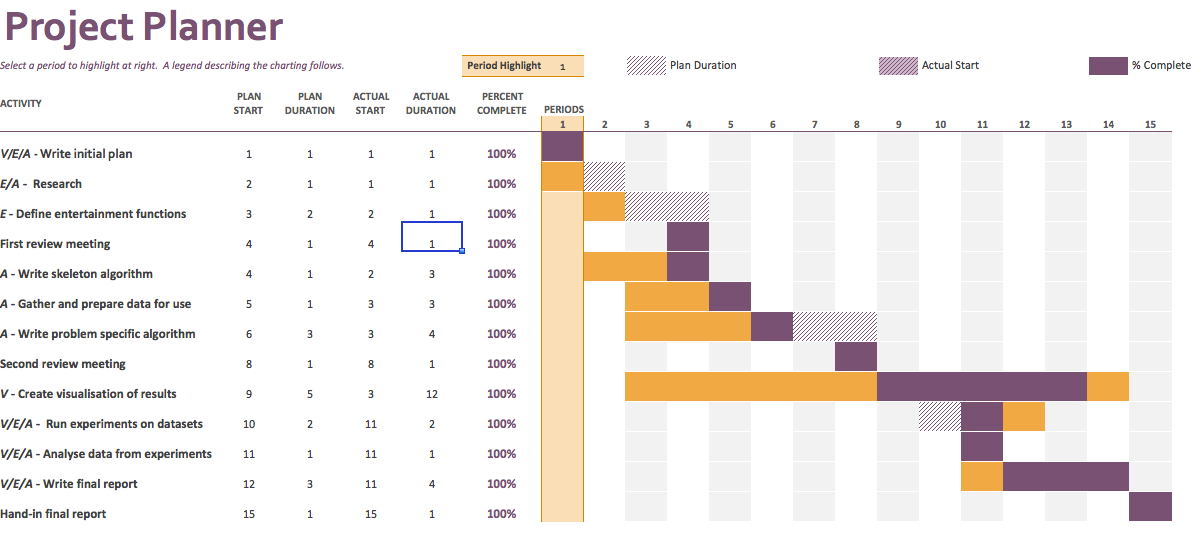
\includegraphics[height=14.5cm, width=\linewidth]{./FinalPlanWorkChart}
\end{figure}
\end{landscape}

\clearpage
\renewcommand{\bibsection}{\section*{References}}
\addcontentsline{toc}{section}{References}
\bibliography{./References/finalReportBib}{}
\bibliographystyle{ieeetr}

\end{document}
